\documentclass[lang=cn,10pt,chinesefont=founder]{elegantbook}

\title{概率论笔记}
%\subtitle{}

\author{肖程哲}
%\institute{}
\date{\today}
%\version{}
%\bioinfo{自定义}{信息}

\extrainfo{苟日新,日日新,又日新}

\setcounter{tocdepth}{3}

\logo{logo.png}
\cover{cover.jpg}

% 本文档命令
\usepackage{array, fdsymbol, tikz}
% 修改标题页的橙色带
% \definecolor{customcolor}{RGB}{32,178,170}
% \colorlet{coverlinecolor}{customcolor}

\tikzset{
box/.style ={
rectangle, %矩形节点
rounded corners =5pt, %圆角
minimum width =50pt, %最小宽度
minimum height =20pt, %最小高度
inner sep=5pt, %文字和边框的距离
draw=blue %边框颜色
}
}

\begin{document}

\maketitle
\frontmatter

\tableofcontents

\mainmatter

\chapter{概率基础}

\begin{introduction}
    \item 事件
    \item 古典概型与几何概率
    \item 条件概率与独立
    \item 乘法法则
    \item 全概率公式
    \item Bayes法则
\end{introduction}

\section{概率空间}

\begin{definition}[样本空间]
    随机试验可能出现的结果称为\textbf{样本点}(sample point),用$\omega$表示。样本的全体构成\textbf{样本空间}(sample space),用$\Omega$表示。
\end{definition}

\begin{definition}[事件的古典定义]
    样本点$\omega$的集合称为\textbf{事件}(event)。
\end{definition}

我们关心的随机现象被抽象为集合, 逻辑运算(且, 或, 非, etc.)对应成集合论运算(交, 并, 补, etc.)。

\begin{property}
    集合的运算性质:
    \begin{description}
        \item [交换律] $A \cup B = B \cup A, \quad AB = BA$
        \item [结合律] $(A \cup B) \cup C = A \cup (B \cup C), (AB)C = A(BC)$
        \item [分配律]
              \begin{gather}
                  (A \cup B) \cup C = A \cup (B \cup C),\\
                  (A \cap B) \cup C = (A \cup C) \cap (B \cup C).
              \end{gather}
        \item [对偶律(De Morgan's laws)]
              \begin{gather}
                  \text{事件并的对立等于对立的交:} \quad \overline{A \cup B} = \overline{A} \cap \overline{B},\\
                  \text{事件交的对立等于对立的并:} \quad \overline{A \cap B} = \overline{A} \cup \overline{B}.
              \end{gather}
    \end{description}
\end{property}

为方便概率的定义,并不把$\Omega$的一切子集作为事件,应避免不可测集的出现。

\begin{definition}[事件域]
    事件构成的全体称为\textbf{事件域}$\mathscr{F}$,是$\Omega$的子集族(collection of subsets),应满足\underline{\,$\sigma$代数}的要求:
    \begin{itemize}
        \item $\emptyset \in \mathscr{F}$, 无事发生;
        \item $A\in\mathscr{F} \implies A^{\complement}\in\mathscr{F}$, 即$\mathscr{F}$对补集运算(逻辑上的非)封闭;
        \item $A_{1},\dots,A_{n},\ldots \in \mathscr{F} \implies \bigcap_{n=1}^{\infty}A_{n} \in \mathscr{F}$, 即$\mathscr{F}$对可数交运算(逻辑上的可数多个且)封闭.
    \end{itemize}
\end{definition}

\begin{note}
    可数性是为了在数学上能够恰当地处理\underline{无穷}的概念, 术语中的$\sigma$指的就是\underline{可数并}。由对偶原理可得$\sigma$域同时对可数并运算封闭. 即$\sigma$域对逆, 并, 交, 差的可数次运算封闭.
\end{note}

事件域根据问题的不同要求适当选取, 在概率定义没有困难时, 应尽量选大, 通常以$\Omega$的一切子集作为事件域. 当$\Omega$给定后,若某些子集必须作为事件处理, 能否找到包含他们的$\sigma$域?

\begin{proposition}
    若给定$\Omega$的一个非空集族$\mathscr{G}$, 必存在$\Omega$上唯一的$\sigma$域$\mathfrak{m}(\mathscr{G})$, 满足下列性质:
    \begin{itemize}
        \item 包含$\mathscr{G}$
        \item 若其他$\sigma$域包含$\mathscr{G}$, 则必包含$\mathfrak{m}(\mathscr{G})$
    \end{itemize}
    这个$\mathfrak{m}(\mathscr{G})$称为包含$\mathscr{G}$的最小$\sigma$域, 或由$\mathscr{G}$扩张而成的$\sigma$域.
\end{proposition}

\emph{扩张}, 或者称为\emph{延拓}, 是数学中很重要的一个概念, 大抵是将某映射的定义域适当扩大, 不改变在初始定义域上的映射取值(注意值域可能是比较抽象的集合, 配备了某些操作之后被称为空间), 同时在扩大后的定义域上仍然保持某些优良的性质. 与此相对的概念是\emph{限制}, 即关心局部上可能更加漂亮的性质, 把初始的定义域适当缩小.

\begin{proof}
    由于$\Sigma$的一切子集构成的集类包含$\mathscr{G}$, 所以$\mathfrak{m}$存在. 再取$\Sigma$上满足此条件的$\sigma$域之交作为$\mathfrak{m}(\mathscr{G})$即可.
\end{proof}

\begin{definition}[Borel集]
    设$\mathbb{R}^1$为全集, 形为$[a,b)$构成的集类产生的$\sigma$域称为\textbf{一维Borel$\sigma$域}, 记为$\mathscr{B}_1$, 其中的元素称为\textbf{一维Borel集}
\end{definition}

若$x,y$为任意实数,由于:
\begin{align*}
    \{x\}  & =  \bigcap_{n=1}^{\infty}\left[x, x+\frac{1}{n}\right) \\
    (x, y) & =  [x, y)-\{x\}                                        \\
    [x, y] & =  [x, y)+\{y\}                                        \\
    (x, y] & =  [x, y)+\{y\}-\{x\}
\end{align*}
因此$\mathscr{B}_1$包含一切开区间, 闭区间, 单个实数, 可列个实数, 以及他们经可列次逆, 并, 交, 差运算的集合.

\begin{definition}[概率空间]
    定义在\underline{事件域}(非样本空间)上的集合函数$P : \mathscr{F} \to \mathbb{R}$称为\textbf{概率}的条件是:
    \begin{description}
        \item[非负性] $P(A)\ge 0 , \forall A \in \mathscr{F}$
        \item[规范性] $P(\Omega) = 1$; (如果没有这条就是一般的{\color{lightgray}有限}\emph{测度})
        \item[可列可加性] 若$A_{1},\dots,A_{n},\ldots \in \mathscr{F}$两两不交, 即$A_{i}\cap A_{j} = \emptyset, \ \forall i\neq j$, 则$P(\bigcup_{n=1}^{\infty}A_{n}) = \sum_{n=1}^{\infty}P(A_{n})$.
    \end{description}
    我们称$(\Omega,\mathscr{F},P)$为一个\textbf{概率空间}(probability space)
\end{definition}

\begin{property}
    概率的性质:
    \begin{itemize}
        \item $P(\Omega)=1$;
        \item $P(A^{\complement})=1-P(A)$;
        \item 若$A \subseteq B $ 则 $P(A)\le P(B)$;
    \end{itemize}
\end{property}

\begin{corollary}[加法公式]
    基础形式:
    \[ P(A \cup B) = P(A) + P(B) - P(AB) \]
    一般形式:
    \begin{align*}
         & P\left(A_{1} \cup A_{2} \cup \cdots \cup A_{n}\right) =  \sum_{i=1, \cdots, n} P\left(A_{i}\right)-\sum_{\substack{i<j \\
        i, j=1, \cdots, n}} P\left(A_{i} A_{j}\right)                                                                             \\
         & +\sum_{\substack{i<j<k                                                                                                 \\i, j, k=1, \cdots, n}} P\left(A_{i} A_{j} A_{k}\right)-\cdots+(-1)^{n-1} P\left(A_{1} A_{2} \cdots A_{n}\right)
    \end{align*}
    特别地, 若事件出现个数相同时概率相等,则可简化为:
    \[ P\left(A_{1} \cup A_{2} \cup \cdots \cup A_{n}\right)=n P_{1} - \binom{n}{2} P_{2} + \binom{n}{3} P_{3}- \cdots+(-1)^{n-1} P_{n} \]
\end{corollary}

显然,可列可加性可以推出有限可加性. 但是一般来讲,由有限可加性并不能推出可列可加性. 设$A_i \in \mathscr{F}, i=1,2,\cdots $且两两互不相容, 若希望由有限可加性推出可列可加性,则需要下式成立:
\[ \lim_{n \to \infty}P(\sum_{i=1}^n A_i) =P(\lim_{n \to \infty}\sum_{i=1}^{n} A_i) \]

\begin{definition}
    对于$\mathscr{F}$上的集合函数$P$,若它对$\mathscr{F}$中任何一个单调不减的集序列$\{ S_n \}$(即$ S_n \in \mathscr{F}, S_n \subseteq  S_{n+1} $)均满足:
    \[ \lim_{n \to \infty}P(S_n) =P(\lim_{n \to \infty} S_n) \]
    则称它是\textbf{下连续的}.
\end{definition}

故若令$S_n = \sum_{i=1}^n A_n$, 则可列可加性条件等价于有限可加性加下连续.

\section{古典概型与几何概率}

\section{条件概率}

\begin{definition}[条件概率]
    令$A,B \in \mathscr{F}$, 且$P(B)>0$称
    \[ P(A|B) = \frac{P(A \cap B)}{P(B)}\]
    为\textbf{基于于$B$的条件概率}(probability conditional on $B$), 这仍然是一个概率测度.
\end{definition}

\begin{theorem}[乘法法则]
    令$A,B \in \mathscr{F}$, 且$P(B)>0$, 则
    \[ P(A \cap B) = P(A|B)P(B) \]
    泛化后有:
    \[ P(A_1 \cap A_2 \cap \cdots \cap A_n) = P(A_{1})P(A_2|A_1)P(A_3|A_1\cap A_2) \cdots  \]
\end{theorem}

\begin{theorem}[全概率公式]
    设 $B_1, B_2, \dotsc, B_n$ 为样本空间 $\Omega$ 的一个分割, 且互不相容, 即$\bigcup _{i=1} ^n B_i = \Omega, B_i B_j= \emptyset for i \neq j $
    如果 $P(B_i) > 0$, $i=1, 2, \dotsc, n$,
    则对任一事件 $A$ 有
    \begin{equation}
        P(A) = \sum_{i=1}^n P(B_i) P(A | B_i).
    \end{equation}
\end{theorem}

\begin{note}
    $P(A | B_i)$可视为事件$A$在$B_i$上的平均, $P(B_i)$则为其权重.
\end{note}

\begin{theorem}[Bayes定理]
    设 $B_1, B_2, \dotsc, B_n$ 为样本空间 $\Omega$ 的一个分割, 且互不相容, 即$\bigcup _{i=1} ^n B_i = \Omega, B_i B_j= \emptyset for i \neq j $
    如果 $P(A) > 0$, $P(B_i) > 0$, $i = 1,2, \dotsc, n$,
    则
    \begin{equation}
        P (B_i | A) = \frac{P(B_i) P(A|B_i)}{\sum_{j=1}^n P(B_j) P(A|B_j)}
    \end{equation}
\end{theorem}

\begin{definition}[事件的独立性]
    如果$A,B\in\mathscr{F}$满足
    \[ P(A\cap B) = P(A)P(B), \]
    则称$A$与$B$\textbf{独立}(independent), 记为$A \Vbar B$.

    对于事件集$A_1, A_2, \dotsc, A_n$, 若对于其中任意子集$A_{i_1}, A_{i_2}, \dotsc, A_{i_n}$有:
    \[ P(A_{i_1} \cap \cdots  \cap A_{i_n}) =P(A_{i_1})\cdots P(A_{i_n})  \]
    则称此事件集\textbf{相互独立}(mutually independent)
\end{definition}

\begin{note}
    当$P(A)>0$时, 我们有$ P(B|A) = P(B) \iff B \Vbar A$, 由此可得到\underline{$B$独立于$A$}的直观理解
\end{note}

\begin{property}
    独立性是对称的, 即$A \Vbar B \iff B \Vbar A$. 若两事件独立, 则其补集也独立.
    \begin{center}
        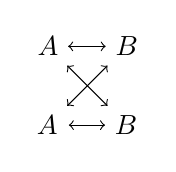
\begin{tikzpicture}
            \node[draw=none,fill=none] (1) at(0,0) {$A^{\complement}$};
            \node[draw=none,fill=none] (2) at(1,0) {$B^{\complement}$};
            \node[draw=none,fill=none] (3) at(0,1) {$A$};
            \node[draw=none,fill=none] (4) at(1,1) {$B$};
            \draw[<->] (1)--(2);
            \draw[<->] (1)--(4);
            \draw[<->] (3)--(2);
            \draw[<->] (3)--(4);
        \end{tikzpicture}
    \end{center}
\end{property}

\begin{definition}[事件域的独立性]
    若$\mathscr{G} \subset \mathscr{F}$与$\mathscr{H} \subset \mathscr{F}$满足
    \[ A \Vbar B, \quad \forall A\in\mathscr{G},\ B\in\mathscr{H}, \]
    则称$\mathscr{G}$与$\mathscr{H}$独立, 记为$\mathscr{G} \Vbar \mathscr{H}$
\end{definition}

测度论告诉我们一个重要结果: 如果$\mathscr{G}$对交集运算封闭, 那么成立$\mathscr{G}\Vbar\mathscr{H} \implies \sigma(\mathscr{G}) \Vbar \mathscr{H}$


\chapter{随机变量}

\begin{introduction}
    \item 离散与连续随机变量
    \item 一元与多元
    \item cdf, pmf, pdf
    \item 条件分布
    \item 独立随机变量
    \item 随机变量函数的分布
    \item 次序随机变量
\end{introduction}

在概率论中,主要关心$X$取值于数值集合$\mathcal{X}$中某个子集$B$的可能性, 即希望得到$\P(\{\omega\in\Omega : X(\omega) \in B\})$. 概率论不关心具体的样本点$\omega\in\Omega$, 将其记为$\{X \in B\} = X^{-1}(B)$. 由于$\P$定义在$\mathscr{F}$上, 故需$X^{-1}(B) \in \mathscr{F}$.

\begin{definition}[可测性]
    设所有值得关心的$B\subset \mathcal{X}$组成$\mathscr{F}_{\mathcal{X}}$, 且$\forall B \in \mathscr{F}_{\mathcal{X}}$都满足$\{X\in B\} \in \mathscr{F}$, 则称$X$为$\mathscr{F}/\mathscr{F}_{\mathcal{X}}$\textbf{可测的}. 当$\mathscr{F}_{\mathcal{X}}$不引起混淆时, 简记为关于$\mathscr{F}$\textbf{可测}, 写作$X \in \mathscr{F}$.
\end{definition}

由于原像保持交、并、补等集合运算, 且$\mathscr{F}$是$\sigma$代数, 可将$\mathscr{F}_{\mathcal{X}}$扩张为合适的最小的$\sigma$代数, 即$\sigma(\mathscr{F}_{\mathcal{X}})$, 因此可测映射的定义不妨\underline{只考虑$\mathscr{F}_{\mathcal{X}}$是$\sigma$代数}的情况.

\begin{definition}[随机变量]
    为了表示因随机性而变动的量, 称\underline{可测映射}(measurable mapping)
    \[ X : (\Omega,\mathscr{F},\P) \to (\mathcal{X},\mathscr{F}_{\mathcal{X}}), \quad \omega\in\Omega \mapsto X(\omega)\in\mathcal{X} \]
    为\textbf{随机元}(random element), 也称\textbf{随机变量}(random variable). 其中$\mathscr{F}_{\mathcal{X}}$
\end{definition}

由于只考虑$\mathscr{F}_{\mathcal{X}}$是$\sigma$代数的情况, 可将随机变量看作将原概率空间映射到新概率空间的方式. 新样本空间由\underline{Borel点集}构成, 对应的概率测度等于原像的.

\begin{remark}
    使用随机变量$X$时, 有两个可能的含义:
    \begin{itemize}
        \item $X$的(随机)取值
        \item $X$的分布
    \end{itemize}
\end{remark}

\begin{definition}[离散与连续随机变量]
    当$\mathcal{X}$是 (至多可数的) 离散点集, $\mathscr{F}_{\mathcal{X}}$由$\mathcal{X}$的所有子集组成, 则称其为\textbf{离散随机变量}(discrete random varible). 当随机变量$\mathcal{X} = \R^{n}$, 考虑$\mathscr{F}_{\mathcal{X}}$为$\left\{\prod_{i=1}^{n}(-\infty,x_{i}] : x_{1},\dots,x_{n}\in\R\right\}$生成的Borel代数(最小的$\sigma$代数), 则称其为\textbf{连续随机变量}(continuous random varible).
\end{definition}

\section{随机变量的分布}

\begin{definition}
    称随机元$X$诱导的\underline{概率测度}
    \[ \P\{X\in\bullet\},\ \bullet\in\mathscr{F}_{\mathcal{X}} \]
    为$X$的\textbf{概率分布}(distribution/law)
\end{definition}
\begin{remark}
    对于随机变量, 他的取值是随机的, 但他的分布是固定的
\end{remark}

\begin{definition}[单变量分布函数]
    一个函数$F : \R \to [0,1]$称为一个单变量分布函数,当其满足以下性质时:
    \begin{description}
        \item[单调性] $F(x_1)\le F(x_2) , \quad \forall x_1<x_2$
        \item[右连续性] $\lim_{x \to x_0^+}F(x)=F(x_0)$
        \item[有界性] $\lim_{n \to -\infty}F(x)=0, \quad \lim_{n \to \infty}F(x)=1$
    \end{description}
\end{definition}

\begin{property}
    $F(x)$最多只有可数个间断点
\end{property}

\begin{proposition}
    对每个分布$Q: \mathscr{B}_1 \to [0,1]$都存在唯一一个分布函数$F_Q : \R \to [0,1]$使得$F_Q(x)=Q[(-\infty,x]], \quad \forall x \in \R$成立。
\end{proposition}

\begin{proposition}
    对每个分布函数$F : \R \to [0,1]$都存在唯一一个分布$Q_F: \mathscr{B}_1 \to [0,1]$使得$Q_F[(-\infty,x]]=F(x), \quad \forall x \in \R$成立。
\end{proposition}

\begin{theorem}
    分布函数可以唯一决定概率分布, 即:
    \[ Q_{F_Q}=Q, \quad F_{Q_F}=F \]
    把随机变量$X$服从分布函数$F(x)$简记作$X \thicksim F(x)$
\end{theorem}

\begin{table}[h]
    \centering
    \begin{tabular}{|c|cc|}
        \hline
                                      & \multicolumn{1}{c|}{离散}                                 & 连续                        \\ \hline
        \multirow{3}{*}{一元随机变量} & \multicolumn{1}{c|}{概率质量函数(pmf)}                    & 概率密度函数(pdf)           \\ \cline{2-3}
                                      & \multicolumn{2}{c|}{累积分布函数(cdf)}                                                  \\ \cline{2-3}
                                      & \multicolumn{2}{c|}{矩母函数/特征函数(mgf/chf)}                                         \\ \hline
        \multirow{3}{*}{多元随机变量} & \multicolumn{1}{c|}{联合概率质量函数(joint pmf)}          & 联合概率密度函数(joint pdf) \\ \cline{2-3}
                                      & \multicolumn{2}{c|}{联合累积分布函数(joint cdf)}                                        \\ \cline{2-3}
                                      & \multicolumn{2}{c|}{联合矩母函数/特征函数(joint mgf/chf)}                               \\ \hline
    \end{tabular}
\end{table}

\begin{definition}[累积分布函数]
    此时$X = (X_{1},\dots,X_{n})^{\top}$的分布由(累积)\textbf{分布函数}(cumulative distribution function, c.d.f.)
    \[ F_{X}(x_{1},\dots,x_{n}) = \P\{X_{1}\leq x_{1},\dots, X_{n}\leq x_{n}\}, \quad x_{1},\dots,x_{n}\in\R. \]
    唯一刻画. 把随机变量$X$服从分布函数$F(x)$简记作$X \thicksim F(x)$
\end{definition}

\begin{figure}[h]
    \centering
    \includegraphics[width=0.8\textwidth]{image/cdf.png}
\end{figure}

\begin{definition}[概率质量函数]
    当且仅当函数$p(x)$满足下述条件时, 被称为\textbf{概率质量函数}(probability mass function, p.m.f.):
    \begin{itemize}
        \item $p(x)\ge 0$
        \item $\sum_{x \in \X}p(x)=1$
    \end{itemize}
\end{definition}

当$X$是离散型随机变量, 设$\mathscr{F}_{\mathcal{X}}$由$\mathcal{X}$的所有子集组成, 此时$X$的分布由
\[ p_{X}(x) = \P\{X=x\} = \P(\{\omega\in\Omega:X(\omega)=x\}), \quad x\in\mathcal{X} \]
唯一刻画. 其与分布函数间的关系为:
\begin{itemize}
    \item $F(x) = \sum_{t\le x}P(X=t)=\sum_{t\le x}p(t)$
    \item $p(x)=P(X=x)=F(x)-F(x-)$
\end{itemize}

\begin{definition}[概率密度函数]
    当且仅当函数$f(x)$满足下述条件时, 被称为\textbf{概率密度函数}(probability density function, p.d.f.):
    \begin{itemize}
        \item $f(x)\ge 0$
        \item $\int_{-\infty}^{\infty}f(x)=1$
    \end{itemize}
\end{definition}

当$X$是连续型随机变量, 且$F_{X} : \R^{n} \to [0,1]$可微(或者更一般地, \underline{绝对连续}), 此时$X$的分布由
\[ f_{X} := \frac{\partial^{n} F_{X}}{\partial x_{1} \cdots \partial x_{n}} \]
唯一刻画. 其与分布函数间的关系为:
\begin{itemize}
    \item $F(x) = \int_{-\infty}^x f(t)dt$
    \item $f(x)=\frac{d}{dx}F(x)$
\end{itemize}

\begin{remark}
    即使对于$f(x)>0$的$x$, $P(X=x)=x\int_{x}^x f(t)dt=0$, 即连续型随机变量在实轴上任意一点的概率测度为零. 概率密度函数$f(x)$代表的是在此位置上单位长度的概率, 可能是一个很大的值.
\end{remark}

\section{多元随机变量}

\begin{definition}[随机向量]
    若随机变量$X_1(\omega), X_2(\omega),\cdots , X_n(\omega)$定义在\underline{同一概率空间}$(\Omega,\mathscr{F},\P)$上, 则称
    \[ X(\omega) = (X_1(\omega), X_2(\omega),\cdots , X_n(\omega)) \]
    构成一个n维\textbf{随机向量},亦称n维随机变量.
\end{definition}

\begin{proposition}
    若$B_n$为$\R^n$上任一博雷尔点集,有
    \[ \{ X(\omega) \in B_n \} \in \mathscr{F} \]
\end{proposition}

\begin{definition}
    称n元函数
    \[ F(x_1,x_2, \cdots , X_n)=\P \{ X_1(\omega)<x_1, X_2(\omega)<x_2,\cdots , X_n(\omega)<x_n \} \]
    为随机向量$X(\omega)$的\textbf{联合分布函数}(joint cdf).
\end{definition}

当$n=2$时,有
\begin{equation}\label{equ:2dim_Prob}
\P((a_1,b_1)\le X < (a_2,b_2))=F(b_1,b_2)-F(a_1,b_2)-F(b_1,a_2)+F(a_1,a_2)
\end{equation}

\begin{property}
    多元分布函数的一些性质:
    \begin{enumerate}
        \item 单调性:关千每个变元是单调不减函数;
        \item \begin{align*}
                  F(x_1,x_2, \cdots, -\infty, \cdots, X_n)=0 \\
                  F(+\infty,+\infty, \cdots, , +\infty)=1
              \end{align*}
        \item 关于每个变元右连续.
        \item 在二元场合,还应该有:对任意$ a_1 <b,,a_2<b_2$ ,都有
              \[ F(b_1,b_2)-F(a_1,b_2)-F(b_1,a_2)+F(a_1,a_2)\ge 0   \]
    \end{enumerate}
\end{property}

为保证\ref{equ:2dim_Prob}式中的概率的非负性,性质4是必须的,而且由性质4可以推出单调性,但存在着反例说明,由单调性并不能保证性质4的成立(见习题 12) .这是多元场合与一元场合的不同之处.

\subsection{边际分布}

\begin{definition}
    对于多维随机变量$X$, 只考虑其中一个分量的分布时, 称其为$X$的\textbf{边际分布或边缘分布}. 对于分量$X_i$, 其\textbf{边缘分布函数}(marginal cdf)为:
    \[ F_{X_i}(x_i) = \P\{ X_i \le x_i \} = F(\infty,\cdots , x_i ,\cdots ,\infty)\] 
\end{definition}



\subsection{独立}

\begin{definition}[独立随机变量]
    若随机变量$X(\omega) = (X_1(\omega), X_2(\omega),\cdots , X_n(\omega))$联合分布函数可分解成各分量边缘分布函数的乘积, 即:
    \[ F(x_1,x_2,\cdots ,x_n) = F_{X_1}(x_1)F_{X_2}(x_2)\cdots F_{X_n}(x_n) , \quad \forall x_1,x_2,\cdots ,x_n \in \R \] 
    则称随机变量$X$各分量相互\textbf{独立}
\end{definition}

\begin{remark}
    对于一般的多元随机变量, 其各分量边缘分布不足以描述联合分布的情况. 但若其各分量独立则可以.
\end{remark}

\begin{theorem}
    对于连续情况:
    \begin{align*}
        &F(x_1,x_2,\cdots ,x_n) = F_{X_1}(x_1)F_{X_2}(x_2)\cdots F_{X_n}(x_n) \\
        \Leftrightarrow & f(x_1,x_2,\cdots ,x_n) = f_{X_1}(x_1)f_{X_2}(x_2)\cdots f_{X_n}(x_n)
    \end{align*}
    对于离散情况:
    \begin{align*}
        &F(x_1,x_2,\cdots ,x_n) = F_{X_1}(x_1)F_{X_2}(x_2)\cdots F_{X_n}(x_n) \\
        \Leftrightarrow & p(x_1,x_2,\cdots ,x_n) = p_{X_1}(x_1)p_{X_2}(x_2)\cdots p_{X_n}(x_n)
    \end{align*}
\end{theorem}

\begin{theorem}
    若随机变量$X,Y$独立, 则其变换$Z=g(X), W=h(Y)$也独立.

    泛化情况:若随机向量$\{X\}_n$各分类独立, 则其变换$\{Y\}_n=g(\{X\}_n)$各分类也独立.
\end{theorem}

\subsection{条件分布}

\begin{definition}
	对一切使 $P\left(Y=y_{j}\right)=p_{ \cdot j}=\sum_{i=1}^{+\infty} p_{i j}>0$ 的 $y_j$, 称
	\begin{equation}\label{eq:3.5.1}
		p_{i | j}=P\left(X=x_{i} | Y=y_{j}\right)=\frac{P\left(X=x_{i}, Y=y_{j}\right)}{P\left(Y=y_{j}\right)}
		=\frac{p_{i j}}{p_{\cdot j}}, \quad i=1,2, \ldots
	\end{equation}
	为给定 $Y=y_j$ 条件下 $X$ 的条件分布列. 若$p_X(x)=0$, 则定义其为0.
\end{definition}

设二维连续随机变量 $(X,Y)$ 的联合密度函数为 $p(x,y)$, 边际密度函数为 $p_X(x),p_Y(y)$.

在离散随机变量场合, 其条件分布函数为 $P(X\leq x|Y=y)$. 但是, 因为连续随机变量取某个值的概率为零, 即 $P(Y=y)=0$, 所以无法用条件概率直接计算 $P(X\leq x|Y=y)$, 一个很自然的想法是: 将 $P(X\leq x|Y=y)$ 看成是 $h\to 0$ 时 $P(X\leq x|y\leq Y\leq y+h)$ 的极限, 即
\begin{align*}
	P(X \leq  x | Y=y) & =\lim _{h \to 0} P(X \leq  x | y \leq  Y \leq  y+h)                                                          \\
	                   & =\lim _{h \to 0} \frac{P(X \leq  x, y \leq  Y \leq  y+h)}{P(y \leq  Y \leq  y+h)}                            \\
	                   & =\lim _{h \to 0} \frac{\int_{-\infty}^{x} \int_{y}^{y+h} p(u, v) dv du}{\int_{y}^{y+h} p_{Y}(v) dv} \\
	                   & =\lim _{h \to 0} \frac{\int_{-\infty}^{x} \left\{ \frac{1}{h} \int_{y}^{y+h} p(u, v) dv \right\} du}
	{\frac{1}{h} \int_{y}^{y+h} p_{Y}(v) dv}.
\end{align*}
当 $p_Y(y),p(x,y)$ 在 $y$ 处连续时, 由积分中值定理可得
\begin{align*}
	 & \lim _{h \to 0} \frac{1}{h} \int_{y}^{y+h} p_{Y}(v) dv=p_{Y}(y), \\
	 & \lim _{h \to 0} \frac{1}{h} \int_{y}^{y+h} p(u, v) dv=p(u, y).
\end{align*}
所以
\[
	P(X \leq x | Y=y)=\int_{-\infty}^{x} \frac{p(u, y)}{p_{Y}(y)} du.
\]
至此, 我们可以定义连续随机变量的条件分布如下.

\begin{definition}
	对一切使 $p_Y(y)>0$ 的 $y$, 给定 $Y=y$ 条件下 $X$ 的\textbf{条件分布函数}\index{T!条件分布函数}和
	\textbf{条件密度函数}\index{T!条件密度函数}分别为
	\begin{align}
		 & F(x | y)=\int_{-\infty}^{x} \frac{p(u, y)}{p_{Y}(y)} du,  \\
		 & p(x | y)=\frac{p(x, y)}{p_{Y}(y)}.
	\end{align}
	同理对一切使 $p_Y(y)>0$ 的 $x$, 给定 $X=x$ 条件下 $Y$ 的条件分布函数和条件密度函数分别为
	\begin{align}
		 & F(y | x)=\int_{-\infty}^{y} \frac{p(x, v)}{p_{X}(x)} dv  \\
		 & p(y | x)=\frac{p(x, y)}{p_{X}(x)}.
	\end{align}
\end{definition}

\begin{remark}
    对于每一个\underline{固定的$x$}, $p_{Y|X}(y|x)$是一个关于$y$的概率质量函数; $f_{Y|X}(y|x)$是一个关于$y$的概率密度函数
\end{remark}

与概率三定理的对应:
\begin{description}
    \item[乘法法则] $p_{XY}(x,y)=p_{Y|X}(y|x)p_{X}(x), \quad f_{XY}(x,y)=f_{Y|X}(y|x)f_{X}(x)$
    \item[全概率公式] $p_{Y}(y)=\sum_{x}p_{Y|X}(y|x)p_{X}(x), \quad f_{Y}(y)=\int^{+\infty}_{-\infty}f_{Y|X}(y|x)f_{X}(x)dx$
    \item[Bayes原理]  $p_{X|Y}(x|y)=\frac{p_{Y|X}(y|x)p_{X}(x)}{\sum_{x}p_{Y|X}(y|x)p_{X}(x)}, \quad f_{X|Y}(x|y)=\frac{f_{Y|X}(y|x)f_{X}(x)}{\int^{+\infty}_{-\infty}f_{Y|X}(y|x)f_{X}(x)dx}$
\end{description}

\section{随机变量的函数}

在统计学中,常需要转化原始数据以获取其中信息, 由此引出了研究随机变量的函数的需要. 以下是获取随机变量的函数的分布的方法:

\subsection{事件法}

\begin{theorem}
    设$Y=g(X)$是随机向量$X=(X_1,X_2,\cdots ,X_n)$的函数, 则$Y$的分布由$X$的分布通过下式决定:
    \[ \P\{Y \in B\} = \P\{X \in A\}, \quad A=\{ \omega |g(\omega)\in B\} \] 
\end{theorem}

此法是其他方法的基础, 但使用不便, 常用于离散随机变量.

\begin{example}
    
\end{example}

\subsection{分布函数法}


\chapter{随机变量的数值特征}

\section{期望}

\begin{definition}
    对于实值随机向量$X : (\Omega,\mathscr{F},\P) \to (\R,\mathscr{B}_{\R})$和(可测)函数$g : \Rn \to \R$, 称
    \[ \E[g(X)] = \int_{\Omega} g(X(\omega))\,\d\P(\omega) = \int_{\R} g(x) \,\d F_{X}(x) \]
    为$g(X)$的\textbf{期望}(expectation).
\end{definition}

\begin{remark}
    当$F_{X}(x)$在$x_0$出连续可导时, $\d F_{X}(x_0)=f_{X}(x_0)\d x$; 当$x_0$为其间断点时时, $\d F_{X}(x_0)=p_{X}(x_0)\delta(x_0)\d x$
\end{remark}

期望算子$\E$是一个线性泛函, 仅适用于\underline{可积}的随机变量.

\begin{definition}
    \begin{enumerate}
        \item 当$g(x)=x$时, $\E[g(x)]=\E[X]$称作$X$的\textbf{均值}(mean), 记为$\mu_{X}$
        \item 当$g(x)=(x-\mu_{X})^{2}$时, $\E[g(x)]=\E[(X-\E[X])^{2}]$称作$X$的\textbf{方差}(variance), 记为$\sigma^2_{X}$. 其平方根称作$X$的\textbf{标准差}(standard deviation), 记为$\sigma_{X}$
        \item 当$g(x,y)=(x-\mu_{X})(y-\mu_{Y})$时, $\E[g(X,Y)]=\E[(X-\E[X])(Y-\E[Y])]$称作$X$与$Y$的\textbf{协方差}(covariance), 记为$\Cov(X,Y)$或$\sigma_{XY}$.
        \item 定义$X$与$Y$的\textbf{相关系数}(correlation coefficient)为:$\sigma_{XY}/(\sigma_{X}\sigma_{Y})$, 记为$\Cor(X,Y)$或$\rho_{XY}$. 若$\rho_{XY}=0$, 则称$X$与$Y$不相关
    \end{enumerate}
\end{definition}

\subsection{均值}

\begin{remark}
    \begin{itemize}
        \item 随机变量的均值可看作其加权平均, 权重为其pdf或pmf, 也即其质心. 从大数定律(\ref{chap:limitation})的角度看, 也可解释为其长期均值.
        \item 方差为随机变量距其均值的均方偏差, 刻画了$X$的变动程度
        \item 随机变量的均值与标准差的单位和其本身的相同, 方差的为其平方
    \end{itemize}
\end{remark}

\begin{theorem}
    均值为随机变量的线性映射, 即:
    \[ \E(a+\sum_{i=1}^n b_i X_i)=a+\sum_{i=1}^n b_i\E( X_i) \]
\end{theorem}

\begin{theorem}[]
    若$X,Y$独立,则
    \begin{gather*}
        \E(XY)=\E(X)\E(Y)
        \E(g(X)h(Y))=\E(g(X))\E(h(Y))
    \end{gather*}
\end{theorem}

\begin{remark}
    由于$\E(X/Y)= \E(X)\E(\frac{1}{Y})$, 而$\E(\frac{1}{Y}) \neq \frac{1}{\E(Y)}$, 所以$\E(X/Y)\neq \E(X)/\E(Y)$
\end{remark}

\begin{theorem}
    若$g$为\underline{下凸(convex)函数}, 则$\E[g(X)] \ge g[\E(X)]$; 若$g$为\underline{上凸(concave)函数}, 则$\E[g(X)] \le  g[\E(X)]$;
\end{theorem}

\begin{figure}
    \centering
    \includegraphics{image/trans_mean.png}
\end{figure}

一个重要结果是, 若$g(X) \ge 0$, 则$\E[g(X)] = 0 \implies g(X) \overset{\as}{=} 0$, 即$\P\{g(X)=0\} = 1$. 其证明可通过\textbf{Markov不等式}
\[ \P\{g(X)\ge\e\} \le \E[g(X)]/\e, \quad \forall \e > 0 \]
完成, 其中需要用到概率的\emph{连续性}, 即$\lim\limits_{n\to\infty}A_{n} = A \implies \lim\limits_{n\to\infty}\P(A_{n}) = \P(A)$.

预处理随机变量有两个常用变换:
\begin{itemize}
    \item \textbf{中心化}(centralization) $X \mapsto X-\E{X}$;
    \item \textbf{标准化}(standardization) $X \mapsto \dfrac{X-\E{X}}{\sqrt{\Var(X)}}$.
\end{itemize}

\subsection{方差}

\begin{theorem}
    $\sigma^2_X=\operatorname{Var}(X)=\E[(X-\mu_X)^2]=E(X^2)-\mu_X$
\end{theorem}

\begin{theorem}
    \[ \operatorname{Var}(a+bX)=b^2\operatorname{Var}(X) \]
\end{theorem}

\begin{theorem}
    \[ \operatorname{Var}(a+\sum_{i=1}^n b_i X_i)=\sum_{i=1}^n b_i^2 \operatorname{Var}(X_i)+\mathbf{b}^{\mathrm{T}} \Sigma \mathbf{b}\]
    其中$\Sigma$为协方差矩阵, $\Sigma_{i,j}=\operatorname{Cov}(X_i,X_j)$
\end{theorem}

\begin{theorem}
    若$X_1,\cdots ,X_n$相互独立, 则:
    \[ \operatorname{Var}(\sum_{i=1}^n X_i)=\sum_{i=1}^n\operatorname{Var}( X_i) \]
\end{theorem}

考虑\textbf{均方误差}(mean squared error)
\[ \MSE(X;\theta) = \E[|X-\theta|^{2}], \quad \theta\in\R, \]
通过\textbf{方差偏差分解}(variance-bias decomposition)
\[ \MSE(X;\theta) = \Var(X) + |\E{X}-\theta|^{2} \]
可以说明$\theta\mapsto\MSE(X;\theta)$在$\E{X}$处取到最小值$\Var(X)$.

\emph{投影}(projection)和\emph{正交分解}的思想在各种内积空间中应用广泛, 这里是$\E = \proj{}{\R}$, 概率论中关于子事件域$\mathscr{G}$ (随机元$X$, resp.)的\emph{条件期望}几何直观是$\proj{}{\mathscr{G}}$ ($\proj{}{\sigma(X)}$, resp.), 线性模型$\mathbf{y} = \mathbf{X}\bm{\beta} + \bm{\e}$中\emph{拟合值}为$\hat{\mathbf{y}} = \proj{\mathbf{y}}{\operatorname{Col}(\mathbf{X})}$.

\begin{theorem}[Chebyshev不等式]
    设随机变量$X$的均值与方差分别为:$\mu, \sigma^2$, 则:
    \[ \P(\left| X-\mu \right| >t)\le \frac{\sigma^{2}}{t^{2}} \]
\end{theorem}

\begin{proof}
    设$f(x)$为$X$的概率密度函数, 令$R=\left\{ x:|x-\mu|>t \right\} $
    \begin{align*}
        \P(|x-\mu|>t) & = \int_R 1 \cdot  f(x)\d x \le \int_R \frac{(x-\mu)^2}{t^{2}}f(x) \d x \\
                      & \le \int_{-\infty}^{\infty}\frac{(x-\mu)^2}{t^{2}}f(x) \d x            \\
                      & = \frac{\sigma^{2}}{t^{2}}
    \end{align*}
\end{proof}

\begin{remark}
    若令$t=k\sigma$, 则$\P(\left| X-\mu \right| >k\sigma)\le \frac{1}{k^{2}}$, 即标准差可代表随机变量偏离均值的概率单位距离.
\end{remark}

\begin{corollary}
    \[ \operatorname{Var}(X)=0 \implies P(X=\mu)=1 \]
\end{corollary}

\subsection{协方差}

协方差代表了$X$与$Y$之间的联合变化倾向, 或者说他们间的相关程度, 但其间\underline{未必有}因果关系.

\begin{theorem}
    \[ \operatorname{Cov} (X,Y)=\E[(X-\mu_X)(Y-\mu_Y)]=\E(XY)-\mu_Y \mu_Y \]
\end{theorem}

\begin{theorem}
    \[ \operatorname{Cov}(a+\sum_{i=1}^n b_i X_i,c+\sum_{j=1}^m d_j Y_j) = \sum_{i=1}^n\sum_{j=1}^m b_i d_j \operatorname{Cov}(X_i,Y_i) = \mathbf{b}^{\mathrm{T}}\Sigma \mathbf{d}\]
\end{theorem}

\begin{theorem}
    独立是不相关的\textbf{充分条件}, 但不是必要条件
\end{theorem}

\begin{theorem}
    $-1\le \rho_{XY} \le 1$, 当且仅当$X$与$Y$间为线性关系时取等号
\end{theorem}

\begin{proof}
    %TODO
\end{proof}

\begin{theorem}
    平移与缩放随机变量都不影响其协方差, 即:
    \[ \left| \operatorname{Cov}(a+ b X,c +d Y) \right| = \left| Cor(X,Y) \right|  \]
\end{theorem}

\section{条件期望}

\begin{definition}
    若$h(Y)$在给定$X=x$下的条件分布(定义\ref{def:cond_dist})的数学期望存在,则定义其为\textbf{条件期望}如下:
    \[ E(h(Y)|X=x) =\begin{cases}
            \sum_{y} h(y) p_{Y|X}(y|x),                    & \text{离散情况} \\
            \int_{-\infty}^{+\infty} h(y) f_{Y|X}(y|x) d y & \text{连续情况}
        \end{cases}\]
\end{definition}

\begin{remark}
    条件期望$\E_{Y|X}(Y|x)$是关于给定变量$x$的函数,不随对应变量$Y$本身变动,但其单位与对应变量$Y$相同,可看作一条在$(X,Y)$平面的曲线。
\end{remark}

\begin{theorem}
    若随机变量$X,Y$独立,则:
    \[ \E_{Y|x}(Y|x)=\E_{Y}(Y) \]
\end{theorem}

\begin{proof}
    由\ref{thm:indep_cmf}可知,若随机变量$X,Y$独立,则
    \begin{align*}
        p_{Y|X}(y|x)&=p_{Y}(y) \\
        f_{Y|X}(y|x)&=f_{Y}(y)
    \end{align*}
    所以$\E_{Y|x}(Y|x)=\E_{Y}(Y)$
\end{proof}

由直观感受亦可知:若$X,Y$独立,则$X$不通过任何与$Y$相关的信息,其条件期望亦当与原期望相同。

\begin{note}
    令$g(x)=\E(h(Y)|X=x)$,则$g(X)$是随机变量$X$的变换,也是随机变量,记为$\E(h(Y)|X)$
\end{note}

\begin{theorem}[重期望公式]
    \[ \E_X[\E_{Y|X}(h(Y)|X)] = \E_{Y}[h(Y)] \]
\end{theorem}

\begin{proof}
    %TODO
\end{proof}

\begin{theorem}
    联合期望公式:
    \[ E_{X,Y}=E_X E_{Y|X} = E_Y E_{X|Y} \]
    泛化情况:
    \[ E_{X,Y}[h(X,Y)]=E_X E_{Y|X}[h(X,Y)|X] = E_Y E_{X|Y}[h(X,Y)|Y] \]
\end{theorem}

\begin{theorem}[重方差公式]\label{thm:var_dec}
    随机变量$Y$的方差可作如下分解:
    \[ \operatorname{Var}_Y(Y)=\operatorname{Var}_X[E_{Y|X}(Y|X)] + E_X[\operatorname{Var}_{Y|X}(Y|X)] \]
\end{theorem}

\begin{figure*}
    \centering
    \includegraphics{image/var_dec.png}
\end{figure*}

\begin{corollary}
    \[ \operatorname{Var}_Y(Y) \ge E_X[\operatorname{Var}_{Y|X}(Y|X)] \]
    当且仅当$E_{Y|X}(Y|X)=E_Y(Y)$时取等号
\end{corollary}

\begin{figure*}
    \centering
    \includegraphics{image/var_dec2.png}
\end{figure*}

\begin{corollary}
    \[ \operatorname{Var}_Y(Y) \ge \operatorname{Var}_X[E_{Y|X}(Y|X)] \]
    当且仅当$\operatorname{Var}_{Y|X}(Y|X)=0$,即$\E_{Y|X}(Y|X)=Y$时取等号
\end{corollary}

\begin{figure*}
    \centering
    \includegraphics{image/var_dec3.png}
\end{figure*}

\section{矩母函数与特征函数}

\subsection{矩}

\begin{definition}
    对于随机变量$X$, 定义其$k$阶\textbf{矩}(moment)为$E(X^k)$, 记为$\mu_k$; 定义其$k$阶\textbf{中心矩}(central moment)为$E((X-\mu_X)^k)$, 记为$\upsilon_k$;
\end{definition}

易知矩与中心矩间存在以下关系:
\begin{align*}
    \upsilon_k & =\sum_{i=0}^k \binom{k}{i} \mu_i (-\mu_X)^{n-i}     \\
    \mu_k      & =\sum_{i=0}^k \binom{k}{i} \upsilon_i (\mu_X)^{n-i}
\end{align*}

特别的有:
\begin{align*}
    E(X)                  & =\mu_1                                                         \\
    \operatorname{Var}(X) & =\upsilon_2=\mu_1^2-2\mu_1 \cdot \mu_1 + \mu_2 = \mu_2-\mu_1^2
\end{align*}

\subsection{矩母函数}

\begin{definition}
    对于随机变量$X$, 若下式期望存在:
    \[ M_X(t) = \E(e^{tX}) \]
    则称其为\textbf{矩母函数}(moment generating function, mgf)。
\end{definition}

\begin{remark}
    此表达式等价于对概率质量函数或密度函数作Laplace变换, 当$t$取某些特定值时, 可能不存在. (若$t=0$则永远存在)
\end{remark}

\begin{theorem}
    若当$t$属于一个包含零点的开区间时, 矩母函数一直存在, 则其唯一对应一个概率分布.
\end{theorem}

\begin{theorem}
    若当$t$属于一个包含零点的开区间时, 矩母函数一直存在, 则:
    \[ M_X^{(k)}(0) = E(X^k) \]
\end{theorem}

\begin{remark}
    由此可方便地计算各阶矩, 故称其为矩母函数. 反过来, 若已知各阶矩, 通过Tayler展开式$M_X(t)=\sum_{k=0}^{\infty}\frac{M_X^{(k)}(0)}{k!}t^k$还原矩母函数, 进而得出概率分布.
\end{remark}

\begin{proposition}
    若$a,b$为常数, 则
    \[ M_{a+b X}(t) = e^{a t}M_X(b t) \]
\end{proposition}

\begin{theorem}\label{thm:mgf_sum}
    若$X,Y$独立,则
    \[ M_{X+Y}(t) = M_X(t) M_Y(t) \]

    泛化情况: 若$X_1,\cdots, X_n$相互独立,则
    \[ M_{X_1+\cdots+ X_n} = \prod_{i=1}^n M_{X_i}(t)\]
\end{theorem}

\subsection{联合特征函数}

\begin{definition}
    对于随机变量$X_1,\cdots, X_n$, 若下式期望存在:
    \[ M_{X_1\cdots X_n}(t_1,\cdots ,t_n) = \E(e^{t_1 X_1+\cdots + t_n X_n}) \]
    则称其为\textbf{联合矩母函数}(joint moment generating function, joint mgf)。
\end{definition}

\begin{remark}
    此处为\underline{多元}函数
\end{remark}

\begin{proposition}
    \[ M_{X_i}(t_i) = M_{X_1\cdots X_n}(0,\cdots ,t_i,\cdots ,0) \]
\end{proposition}

\begin{theorem}
    当且仅当:
    \[ M_{X_1\cdots X_n}(t_1,\cdots ,t_n) = \prod_{i=1}^n M_{X_i}(t_i) \]
    时, $X_1,\cdots, X_n$相互独立
\end{theorem}

\begin{remark}
    与\underline{累计函数、密度函数、质量函数}的情况类似,变量相互独立等价于联合函数可拆分为边缘函数的乘积
\end{remark}

\begin{theorem}
    \[ \frac{\partial^{r_1+\cdots +r_n} }{\partial t_1^{r_1} \cdots  \partial t_n^{r_n}} M_{X_1\cdots X_n}(t_1,\cdots ,t_n) = E(X_1^{r_1} \cdots X_n^{r_n}) \]
\end{theorem}

\subsection{特征函数}

由于有时矩母函数可能不存在,为避免此缺陷,构造出与之特性类似的特征函数。

\begin{definition}
    对于随机变量$X$, 定义其\textbf{特征函数}(characat function, chf)为:
    \[ \phi_X(t) = \E(e^{itX}) = \E(\cos (tX)) + i\E(\sin (tX))\]

    对于随机变量$X_1,\cdots, X_n$, 定义其\textbf{联合特征函数}(joint characat function, joint chf)为:
    \[ \phi_{X_1\cdots X_n}(t_1,\cdots ,t_n) = \E(e^{i (t_1 X_1+\cdots + t_n X_n)}) \]
\end{definition}

\begin{remark}
    此表达式等价于对概率质量函数或密度函数作Fourier变换
\end{remark}

\begin{proposition}
    随机变量的特征函数总是存在
\end{proposition}

\begin{proposition}
    若矩母函数存在,则其与特征函数之间满足关系:
    \[ \phi_X(t) = M_X(it) \]
\end{proposition}

\begin{theorem}
    特征函数可通过以下逆变换得到分布:
    \begin{description}
        \item[离散] $p_{X}(x)=\lim _{T \rightarrow \infty} \int_{-T}^{T} e^{-i t x} \phi_{X}(t) d t$
        \item[连续] $f_{X}(x)=\frac{1}{2 \pi} \int_{-\infty}^{\infty} e^{-i t x} \phi_{X}(t) d t$
    \end{description}
\end{theorem}

\section{估计与预测}

\subsection{$\delta$法}

\subsection{预测}




\section{熵与信息}

\chapter{常见分布}
\begin{introduction}[考试重点]
    \item 各分布的特征
    \item 各分布联系与转换
    \item 多维正态分布
\end{introduction}
\section{离散分布}

\subsection{均匀分布}

\begin{definition}[离散均匀分布]
    若随机变量只能在$a_1,\cdots ,a_n$中取值,并且对应的概率相同,则称其遵循\textbf{均匀分布}(Uniform distribution),记为$X \sim U(a_1,\cdots ,a_n)$。
\end{definition}
\begin{remark}
    此即古典概型。
\end{remark}

离散均匀分布的特征:
\begin{description}
    \item[参数] $a_i \in \mathbb{R}$
    \item[概率质量函数] $p(x)=\begin{cases}
                \frac{1}{m} & x=a_1,a_2,\cdots ,a_n \\
                0           & \text{其他}
            \end{cases}$
    \item[矩母函数] $M(t)=\frac{\sum_{i=1}^m e^{a_i t}}{m}$
    \item[均值] $\mu=\frac{\sum_{i=1}^m a_i }{m}=\overline{a}$
    \item[方差] $\sigma^2=\frac{\sum_{i=1}^m (a_i-\overline{a})^2 }{m}$
    \item[实例] 丢一个均匀的骰子
\end{description}

\subsection{两点分布}

\begin{definition}[两点分布]
    若随机变量只能取0或1,并且对应的概率分别为$1-p$与$p$,则称其遵循\textbf{两点分布}(Bernouli distribution)(也称0-1分布、两点分布分布),记为$X \sim B(1,p)$。
\end{definition}

两点分布的特征:
\begin{description}
    \item[参数] $p \in [0,1]$
    \item[概率质量函数] $p(x)=\begin{cases}
                p^x (1-p)^{1-x} & x \in \{0,1 \} \\
                0               & \text{其他}
            \end{cases}$
    \item[矩母函数] $M(t)=p e^t + 1-p$
    \item[均值] $\mu=p$
    \item[方差] $\sigma^2=p(1-p)$
    \item[实例] 丢一次硬币,$p$代表某一面出现的概率
\end{description}

\begin{remark}
    若$A$是一个事件,出现概率为$p_A$,则指示随机变量$I_A$(若$A$出现记为1,否则为0)遵循Bernouli分布,即$I_A \sim B(p_A)$
\end{remark}

\subsection{二项分布}

\begin{definition}[二项分布]\label{def:binom_dist}
    若进行$n$次独立的Bernouli实验(定义\ref{def:Bernouli_experiment})$X_1,\cdots,X_n \overset{\text{i.i.d.}}{\sim} B(1,p)$,则这些随机变量之和$Y=X_1+\cdots+X_n$遵循\textbf{二项分布}(binomial distribution),记为$Y \sim B(n,p)$。
\end{definition}

二项分布的特征:
\begin{description}
    \item[参数] $p \in [0,1], n \in \mathbb{N}_+$
    \item[概率质量函数] $p(x)=\begin{cases}
                \binom{n}{x} p^x (1-p)^{n-x} & x \in \mathbb{N}^n \\
                0                            & \text{其他}
            \end{cases}$
    \item[矩母函数] $M(t)=(p e^t + 1-p)^n$,求解方法有:
        \begin{itemize}
            \item \underline{独立变量}之和的矩母函数等于各变量矩母函数之积(定理\ref{thm:mgf_sum})
            \item 定义
        \end{itemize}
    \item[均值] $\mu=np$,求解方法有:
        \begin{itemize}
            \item 定义(例\ref{ex:binom_dist_mean})
            \item 矩母函数在$t=0$的一阶导
            \item 变量之和的均值等于各变量均值之和
        \end{itemize}
    \item[方差] $\sigma^2=np(1-p)$,求解方法有:
        \begin{itemize}
            \item 定义(例\ref{ex:binom_dist_var})
            \item 矩母函数在$t=0$的二阶导,$\operatorname{Var}(X)=E(X^2)-(E(X))^2$
            \item \underline{独立变量}之和的方差等于各变量均值之和
        \end{itemize}
    \item[实例] 丢$n$次硬币,$p$代表某一面出现的概率,出现此面的次数
\end{description}

\begin{figure}[!ht]
    \centering
    \raisebox{0.75cm}{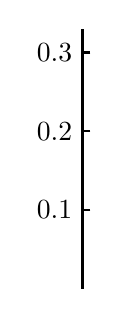
\begin{tikzpicture}[thick]
            \draw(0,0.3)--(0,3.6);
            \draw(0.1,1.3)--(0,1.3)node[left]{$0.1$}
            (0.1,2.3)--(0,2.3)node[left]{$0.2$}
            (0.1,3.3)--(0,3.3)node[left]{$0.3$};
        \end{tikzpicture}}
    \subfloat[$b(10,0,2)$的线条图(右偏)]{
        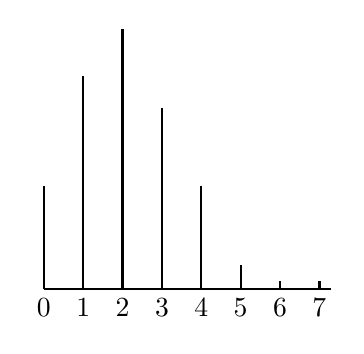
\begin{tikzpicture}[thick,xscale=0.5]
            \draw(0,0)node[below]{$0$}--(0,1.3)(1,0)node[below]{$1$}--(1,2.7)
            (2,0)node[below]{$2$}--(2,3.3)(3,0)node[below]{$3$}--(3,2.3)
            (4,0)node[below]{$4$}--(4,1.3)(5,0)node[below]{$5$}--(5,0.3)
            (6,0)node[below]{$6$}--(6,0.1)(7,0)node[below]{$7$}--(7,0.1);
            \draw(0,0)--(7.3,0);
        \end{tikzpicture}
    }\hfill
    \subfloat[$b(10,0,5)$的线条图(对称)]{
        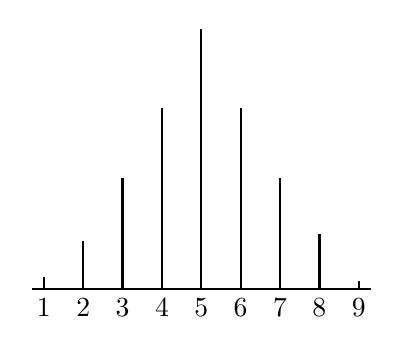
\begin{tikzpicture}[thick,xscale=0.5]
            \draw(1,0)node[below]{$1$}--(1,0.15)(2,0)node[below]{$2$}--(2,0.6)
            (3,0)node[below]{$3$}--(3,1.4)(4,0)node[below]{$4$}--(4,2.3)
            (5,0)node[below]{$5$}--(5,3.3)(6,0)node[below]{$6$}--(6,2.3)
            (7,0)node[below]{$7$}--(7,1.4)(8,0)node[below]{$8$}--(8,0.7)
            (9,0)node[below]{$9$}--(9,0.1);
            \draw(0.7,0)--(9.3,0);
        \end{tikzpicture}
    }\hfill
    \subfloat[$b(10,0,8)$的线条图(左偏)]{
        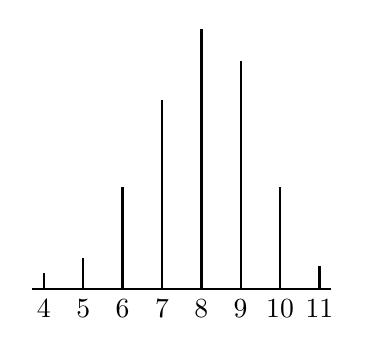
\begin{tikzpicture}[thick,xscale=0.5]
            \draw(4,0)node[below]{$4$}--(4,0.2)(5,0)node[below]{$5$}--(5,0.4)
            (6,0)node[below]{$6$}--(6,1.3)(7,0)node[below]{$7$}--(7,2.4)
            (8,0)node[below]{$8$}--(8,3.3)(9,0)node[below]{$9$}--(9,2.9)
            (10,0)node[below]{$10$}--(10,1.3)(11,0)node[below]{$11$}--(11,0.3);
            \draw(3.7,0)--(11.3,0);
            \draw[very thick](8,0)--(8,3.3);
        \end{tikzpicture}
    }
    \caption{二项分布$b(n,p)$的线条图\label{fig2.4.1}}
\end{figure}

从上图可以看出:
\begin{itemize}
    \item 位于均值$np$附近概率较大;
    \item 随着$p$的增加,分布的峰逐渐右移.
\end{itemize}

\begin{proposition}
    二项分布之和仍是二项分布。若$X_1+\cdots+X_k$独立且$X_i \sim B(n_i,p)$,则$Y=X_1+\cdots+X_k  \sim B(n_1+\cdots+n_k,p )$
\end{proposition}

\subsection{泊松分布}

\begin{theorem}[Poisson逼近]\label{thm:Poisson_theorem}
    \[ \lim_{n p_n \to \lambda} \binom{n}{k} p_n^{k} (1-p_n)^{n-k} = \frac{\lambda^{k}}{k !}e^{-\lambda} \]
\end{theorem}
\begin{proof}
    记$np_n=\lambda_n$,记$p_n=\lambda_n/n$,我们可得
    \begin{align*}
        \binom {n}{k} p_n^k(1-p_n)^{n-k} & = \frac{n(n-1)\cdots(n-k+1)}{k!}\left( \frac{\lambda_n}n \right)^k \left( 1 - \frac{\lambda_n}n \right)^{n-k} \\
                                         & = \frac{\lambda_n^k}{k!}\left( 1 - \frac1n \right)\left( 1 - \frac2n \right) \cdots
        \left( 1 - \frac{k-1}n \right)
        \left( 1 - \frac{\lambda_n}n \right)^{n-k}.
    \end{align*}
    对固定的$k$有
    \[ \lim_{n\to+\infty}\lambda_n = \lambda,\ \lim_{n\to+\infty}\left( 1 - \frac{\lambda_n}n \right)^{n-k} = e^{-\lambda},\ \lim_{n\to+\infty}\left( 1 - \frac{1}{n} \right) \cdots \left( 1 - \frac{k-1}n \right) = 1 \]
    从而
    \[ \lim_{n\to+\infty} \binom{n}{k} p_n^k(1-p_n)^{n-k}  = \frac{\lambda^k}{k!}e^{-\lambda} ,\ \forall k \in \mathbb{N}\]
\end{proof}

\begin{definition}[Poisson分布]
    若随机变量$X$的概率分布列满足以下形式:
    \[ P(X = k) = \frac{\lambda^k}{k!}e^{-\lambda},\ k \in \mathbb{N} \]
    则称其遵循\textbf{Poisson分布},记为$X \sim P(\lambda)$.
\end{definition}

\begin{remark}
    由定理\ref{thm:Poisson_theorem}可看出,Poisson分布可作为二项分布的近似。$\lambda$的涵义%TODO
\end{remark}

Poisson分布的特征:
\begin{description}
    \item[参数] $\lambda>0$
    \item[概率质量函数] $p(k)=\begin{cases}
                \frac{\lambda^{k}}{k !}e^{-\lambda} & x \in \mathbb{N}^n \\
                0                                   & \text{其他}
            \end{cases}$
    \item[矩母函数] $M(t)=e^{\lambda (e^t -1)}$,求解方法有:
        \begin{itemize}
            \item 利用公式
            \item 凑一法
        \end{itemize}
    \item[均值] $\mu=\lambda$
    \item[方差] $\sigma^2=\lambda$
    \item[实例] 公共汽车站来到的乘客数
\end{description}

\begin{proposition}
    Poisson分布之和仍是Poisson分布。若$X_1+\cdots+X_k \overset{\text{i.i.d.}}{\sim} P(\lambda_i)$,则$Y=X_1+\cdots+X_k  \sim P(\lambda_1+\cdots+\lambda_k)$
\end{proposition}

\begin{proof}
    \[ M_Y(t)=\prod_i^k M_{X_i}(t)=\exp \{(e^t-1)\sum_{i=1}^k \lambda_i\} \]
\end{proof}

\begin{lemma}\label{lem:Cauchy_lemma}
    若$f(x)$是连续函数(或单调函数),且对一切$x,y$(或一切$x,y\ge 0$)成立:
    \[ f(x)f(y)=f(x+y) \]
    则$f(x)$为\textbf{指数函数}。
\end{lemma}

\begin{proof}
    \begin{align*}
        \because   & f(1)=[f(\frac{1}{n})]^n                           \\
        \text{且}  & a=f(1)=[f(\frac{1}{2})]^2\ge 0                    \\
        \therefore & f(\frac{1}{n})=a^{\frac{1}{n}}                    \\
        \therefore & f(\frac{m}{n})=[f(\frac{1}{n})]^m=a^{\frac{m}{n}}
    \end{align*}
    即此命题对一切有理数成立。又实数具有连续性,故此命题对一切实数成立。
\end{proof}

\begin{definition}[泊松过程]
    若某一随机过程满足以下特征,则称其为\textbf{泊松过程}:
    \begin{description}
        \item[平稳性] 随机事件$A$在$[t_0, t_0 + t)$中的发生次数只与时间间隔长度$t$有关而与时间起点$t_0$无关。将在长度为$t$的时间区间中发生$K$次事件$A$的概率记为$P_k(t)$。
        \item[独立增量性] 在$[t_0, t_0 + t)$中发生$K$次事件$A$的概率与时刻$t_0$以前发生的事件独立。
        \item[普通性] 在充分小的时间间隔中,最多发生一次事件$A$。即,若记$\psi(t)=\sum_{k=2}^{\infty}P_k(t)=1-P_0(t)-P_1(t)$,则有$\lim_{t \to 0}\psi(t)/t=0$
    \end{description}
\end{definition}

对$\Delta t>O$,考虑$[O,t+\Delta t)$中发生$K$次事件$A$的概率$P_k(t+\Delta t)$,由独立增量性及全概率公式可得:
\[ P_k(t+\Delta t)=P_k(t)P_0(\Delta r) + P_{k-1}P_1(\Delta t)+ \cdots +P_0(t)P_k(\Delta t) ,k\ge 0\]
(对$n\ge 1$ ,假定$P_{-n}(t)=0$)

特别地
\[ P_0(t+\Delta t)=P_0(t)P_0(\Delta t) \]
由引理\ref{lem:Cauchy_lemma}知
\[ P_0(t)=a^{t}, a\ge 0 \]
若$a=O$,则$P_0(t) \equiv 0$,说明在不管怎么短的时间间隔内事件$A$都发生,因此在有限时间间隔中将发生无穷多个次事件$A$,这种情形不在我们的考虑之列。此外,因$P_0(t)$是概率,故应有$a\ge 1$,而当$a=1$时,$P_0(t) \equiv 1$,表明事件$A$永不发生,也不是我们感兴趣的情形,所以应有 $0<a<1$,从而存在$\lambda>0$,使
\[ P_0(t)=e^{-\lambda t} \]
因此当$\Delta t \to 0$时,有
\begin{align*}
    P_{0}(\Delta t)                                & =\ee^{-\lambda \Delta t}=1-\lambda \Delta t+o(\Delta t)                  \\
    P_{1}(\Delta t)                                & =1-P_{0}(\Delta t)-\psi(\Delta t)=\lambda \Delta t+o(\Delta t)           \\
    \sum_{l=2}^{\infty} P_{k-l}(t) P_{l}(\Delta t) & \leqslant \sum_{l=2}^{\infty} P_{l}(\Delta t)=\psi(\Delta t)=o(\Delta t) \\
\end{align*}
所以:
\[ P_k(t+\Delta t)=P_k(t)(1-\lambda \Delta t) + P_{k-1}\lambda \Delta t+ o(\Delta t) ,k\ge 1\]
因此:
\[ P'_k(t)= \frac{P_k(t+\Delta t)-P_k(t)}{\Delta t} = \lambda[P_{k-1}-P_k(t)] \]

由于$P_0(t)=\ee^{-\lambda t}$,故有$P'_1(t)=\lambda[\ee^{-\lambda t}-P_1(t)]$,可解得$P_0(t)=\lambda t \ee^{-\lambda t}$,依次可递推可解得:
\[ P_k(t)=\frac{(\lambda t)^k}{k!}\ee^{-\lambda t}, k \in \mathbb{N}\]
正是参数为$\lambda t$的泊松分布。

\subsection{几何分布}

\begin{definition}
    若进行无限次独立的Bernouli实验,则第一次出现“1”的实验次数遵循\textbf{几何分布}(geometric distribution),记为$X \sim G(p)$。
\end{definition}

\begin{figure*}[h]
    \centering
    \includegraphics{image/geometric_dist_intu.png}
\end{figure*}

几何分布的特征:
\begin{description}
    \item[参数] $p \in [0,1]$
    \item[概率质量函数] $p(x)=\begin{cases}
                (1-p)^{x-1} p & x \in \mathbb{N}_+ \\
                0             & \text{其他}
            \end{cases}$
    \item[矩母函数] $M(t)=\frac{p e^t}{1-(1-p)e^t}, t<-\ln (1-p)$,求解方法有:
        \begin{itemize}
            \item \underline{独立变量}之和的矩母函数等于各变量矩母函数之积(参见定理\ref{thm:mgf_sum})
            \item 定义
        \end{itemize}
    \item[均值] $\mu=\frac{1}{p}$,求解方法有:
        \begin{itemize}
            \item $E(X)=\sum_{k=1}^{\infty}P(X\ge k)$(定理\ref{prop:mean_of_non-negative_discrete_varible})
            \item 矩母函数在$t=0$的一阶导
            \item 定义(例\ref{ex:geometric_dist_mean})
        \end{itemize}
    \item[方差] $\sigma^2=\frac{1-p}{p^2}$,求解方法有:
        \begin{itemize}
            \item 定义(例\ref{ex:geometric_dist_var})
            \item 矩母函数在$t=0$的二阶导,$\operatorname{Var}(X)=E(X^2)-(E(X))^2$
        \end{itemize}
    \item[实例] 买彩票时,中奖所需购买张数。
\end{description}

\begin{proposition}
    离散分布中有且只有几何分布具备无记忆性:
    \[ P\{ X>m+n|X>m \} =P\{ X>n \} ,\quad \forall s>0,t>0\]
\end{proposition}
\begin{proof}
    \begin{align*}
        \because   & P(X>n)=\sum_{k=n+1}^{\infty}(1-p)^k p=\frac{p(1-p)^n}{1-(1-p)}=(1-p)^n \\
        \therefore & P\{ X>m+n|X>m \} =P\{ X>n \}=\frac{(1-p)^{m+n}}{(1-p)^m}               \\
                   & =(1-p)^n=P\{ X>n \}
    \end{align*}
    即几何分布具备无记忆性。

    设$X$是取正整数值的随机变量,满足:在已知$X>k$的条件下,$X=k+1$的概率与$k$无关。令$p=P\{ X=k+1|X>k \}$,并记$q_k=P\{ X>k \}$,以及$P_k=P\{ X=k \}$,那么$P_{k+1}=q_k-q_{k+1}$,且
    \[ p=\frac{p_{k+1}}{q_k} \]
    即
    \[ \frac{q_{k+1}}{q_k}=1-p \]
    注意到$q_0=1$,那么$q_k=(l-p)^k$,因此
    \[ p_k=p(l-p)^{k-l},\quad k \in N_+ \]
    正是几何分布
\end{proof}

\subsection{负二项分布}

\begin{definition}
    若进行无限次独立的Bernouli实验,则第$r$次出现“1”的实验次数遵循\textbf{负二项分布}(negative binomial distribution),记为$X \sim NB(r,p)$。
\end{definition}

\begin{figure*}[h]
    \centering
    \includegraphics{image/NB_dist_intu.png}
\end{figure*}

负二项分布的特征:
\begin{description}
    \item[参数] $p \in [0,1]$
    \item[概率质量函数] $p(x)=\begin{cases}
                \binom{x-1}{r-1}p^r (1-p)^{x-r} p & x \in \mathbb{N}_r \\
                0                                 & \text{其他}
            \end{cases}$
    \item[矩母函数] $M(t)=\frac{p^r e^{rt}}{(1-(1-p)e^t)^r}, t<-\ln (1-p)$,求解方法有:
        \begin{itemize}
            \item \underline{独立变量}之和的矩母函数等于各变量矩母函数之积(参见定理\ref{thm:mgf_sum})
            \item 定义凑一法
            \item 利用公式$\sum_{x=0}^{\infty}\binom{n+x-1}{x}t^x=\frac{1}{(1-t)^n},-1<t<1$
        \end{itemize}
    \item[均值] $\mu=\frac{r}{p}$,求解方法有:
        \begin{itemize}
            \item 定义凑一法
            \item 矩母函数在$t=0$的一阶导
            \item 独立几何分布之和(定理\ref{prop:sum_of_geo})
        \end{itemize}
    \item[方差] $\sigma^2=\frac{r(1-p)}{p^2}$,求解方法有:
        \begin{itemize}
            \item 定义(凑一法)
            \item 矩母函数在$t=0$的二阶导,$\operatorname{Var}(X)=E(X^2)-(E(X))^2$
            \item 独立几何分布之和(定理\ref{prop:sum_of_geo})
        \end{itemize}
    \item[实例] 买彩票时,中奖$r$次所需购买张数。
\end{description}

\begin{proposition}\label{prop:sum_of_geo}
    几何分布之和是负二项分布。若$X_1+\cdots+X_r$独立且$X_i \sim G(p)$,则$Y=X_1+\cdots+X_r  \sim NB(r,p)$
\end{proposition}

\begin{proof}
    %TODO 
\end{proof}

\begin{proposition}
    负二项分布之和仍是负二项分布。若$X_1+\cdots+X_k$独立且$X_i \sim NB(r_i,p)$,则$Y=X_1+\cdots+X_k  \sim B(r_1+\cdots+r_k,p )$
\end{proposition}

\begin{proof}
    %TODO 
\end{proof}

\subsection{多项分布}

\begin{definition}[多项分布]
    若进行$n$次独立的实验,每次实验有$r$种结果,每种结果对于概率分别为$p_1,\cdots ,p_r$。令$X_i$代表得出结果$i$的次数,则随机向量$\mathbf{X}=(X_1,\cdots ,X_r)$遵循\textbf{多项分布}(multinomial distribution),记为$\mathbf{X} \sim Multinomial(n,p_1,\cdots ,p_r)$。
\end{definition}

多项分布的特征:
\begin{description}
    \item[参数] $p_i \in [0,1], \sum_{i=1}^r p_i=1$
    \item[概率质量函数] $p(x)=\begin{cases}
                \binom{n}{x_1 \cdots x_r} p_1^{x_1}\cdots p_r^{x_r} & x \in \mathbb{N}^n \& \sum_{i=1}^r x_i=n \\
                0                                                   & \text{其他}
            \end{cases}$
    \item[矩母函数] $M(t_1,\cdots ,t_r)=(p_1 e^{t_1} +\cdots + p_r e^{t_r})^n$,求解方法有:
        \begin{itemize}
            \item 利用公式
            \item 凑一法
        \end{itemize}
    \item[边缘分布] $X_i \sim B(n,p_i)$
    \item[均值] $E(X_i)=np_i$
    \item[方差] $\operatorname{Var}(X_i)=np_i(1-p_i)$
    \item[协方差] $\operatorname{Cov}(X_i,X_j)=-p_i p_j$,求解方法有:
        \begin{itemize}
            \item 矩母函数求解$E(X_i X_j)$
            \item 凑一法求解$E(X_i X_j)$
        \end{itemize}
    \item[实例]
\end{description}

\begin{remark}
    多项分布是二项分布的泛化。
\end{remark}

\subsection{超几何分布}

\begin{definition}
    设有$N$个产品,其中有$M$个不合格品.若从中不放回地随机抽取$n$个,则其中含有的不合格品的个数$X$服从超几何分布,记为$X \sim h(n,N,M)$
\end{definition}

超几何分布的特征:
\begin{description}
    \item[参数] $M,n \le N \quad n,N,M \in N_+$
    \item[概率质量函数] $p(k)=\begin{cases}
                \frac{\binom Mk \binom{N-M}{n-k}} {\binom Nn}  ,\  & k = 0,1,\cdots,r \\
                0                                                  & \text{其他}
            \end{cases}$
    \item[矩母函数] 存在,但没有简单的表达
    \item[均值] $\mu=n\frac{M}{N}$(利用凑一法,例\ref{ex:binom_dist_mean})
    \item[方差] $\sigma^2=\frac{nM(N-M)(N-n)}{N^2(N-1)}$
    \item[实例] 从一个有限总体中进行不放回抽样
\end{description}

\begin{remark}
    若$\frac{n}{N} \to 0$时,$\frac{M}{N} \to p$,则超几何分布可近似为二项分布。
    \[ \frac{\binom {M}{k} \binom{N-M}{n-k}} {\binom {N}{n}} \approx \binom{n}{k}p^k(1-p)^{n-k} ,\quad p=\frac{M}{N} \]
\end{remark}

\section{连续分布}

\subsection{均匀分布}

\begin{definition}
    若随机变量$X$在$[a,b]$中任一区域的概率与其测度成正比,则称$X$服从区间$(a,b)$上的\textbf{均匀分布}(Uniform distribution),记作$X\sim U(a,b)$。
\end{definition}

\begin{figure}[!ht]
    \centering
    \subfloat[密度函数$p(x)$]{
        \begin{tikzpicture}[semithick,>=stealth,samples=100,scale=2.5]
            \draw[->](0,0)node[below left]{$O$}--(1.7,0)node[below]{$x$};
            \draw[->](0,0)--(0,1.2)node[right]{$p(x)$};
            \draw[thick](0.3,0.6)--(1.3,0.6);\node[left]at(0,0.6){$\frac1{b-a}$};
            \draw[dashed](0.3,0.6)--(0.3,0)node[below]{$a$}
            (1.3,0.6)--(1.3,0)node[below]{$b$};
        \end{tikzpicture}
    }
    \subfloat[分布函数$F(x)$]{
        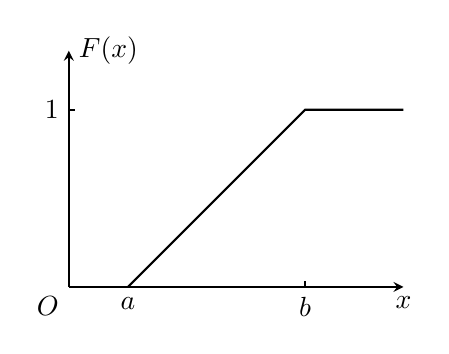
\begin{tikzpicture}[semithick,>=stealth,samples=100,scale=2.5]
            \draw[->](0,0)node[below left]{$O$}--(1.7,0)node[below]{$x$};
            \draw[->](0,0)--(0,1.2)node[right]{$F(x)$};
            \draw[thick](0.3,0)node[below]{$a$}--(1.2,0.9)--(1.7,0.9);
            \draw(1.2,0)node[below]{$b$}--(1.2,0.03);
            \draw(0,0.9)node[left]{$1$}--(0.03,0.9);
        \end{tikzpicture}
    }
    \caption{$(a,b)$上的均匀分布}\label{fig:2.5.3}
\end{figure}

均匀分布的特征:
\begin{description}
    \item[参数] $a<b , \quad a,b \in \mathbb{R} $
    \item[概率质量函数] $p(x)=\begin{cases}
                \frac1{b-a}, & a < x < b   \\
                0            & \text{其他}
            \end{cases}$
    \item[分布函数]  $ F(x) = \begin{cases}
                0,               & x < a ;      \\
                \frac{x-a}{b-a}, & a \le x < b; \\
                1,               & x \ge b.
            \end{cases}$
    \item[矩母函数] $M(t)=\frac{e^{bt}-e^{at}}{t(b-a)} , \quad t \in \mathbb{R}$
    \item[均值] $\mu=\frac{a+b}{2}$
    \item[方差] $\sigma^2=\frac{(b-a)^2}{12}$
\end{description}

\begin{remark}
    常利用$U(0,1)$生成特定分布的伪随机数(参见定理\ref{thm:pseudo_random_generation})
\end{remark}

\subsection{指数分布}

\begin{definition}
    若随机变量X的密度函数(见图 \ref{fig2.5.4})为
    \[ p(x) = \begin{cases}
            \lambda e^{-\lambda x}, & x \ge 0; \\
            0,                      & x < 0,
        \end{cases} \]
    则称$X$服从\textbf{指数分布},记作$X\sim Exp(\lambda)$,其中参数$\lambda>0$. 指数分布的分布函数为
    \[ F(x) = \begin{cases}
            1 - e^{-\lambda x}, & x \ge 0; \\
            0,                  & x < 0.
        \end{cases}\]
\end{definition}

\begin{figure}[!ht]
    \centering
    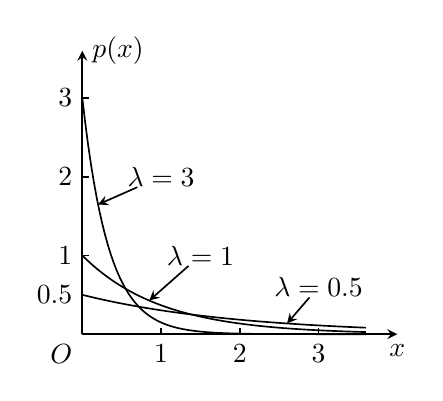
\begin{tikzpicture}[semithick,>=stealth,samples=100]
        \draw[->](0,0)node[below left]{$O$}--(4,0)node[below]{$x$};
        \draw[->](0,0)--(0,3.6)node[right]{$p(x)$};
        \foreach \x in{1,2,3}
        \draw(\x,0)node[below]{$\x$}--(\x,0.08)(0,\x)node[left]{$\x$}--(0.08,\x);
        \draw[domain=0:3.6]plot(\x,{e^(-\x)});
        \draw[domain=0:3.6](0,0.5)node[left]{$0.5$}--plot(\x,{0.5*e^(-0.5*\x)});
        \draw[domain=0:3.6]plot(\x,{3*e^(-3*\x)});
        \node[inner sep=0pt](a)at(1,2){$\lambda=3$};
        \node[inner sep=0pt](b)at(1.5,1){$\lambda=1$};
        \node[inner sep=0pt](c)at(3,0.6){$\lambda=0.5$};
        \draw[->](a)--(0.2,{3*e^(-3*0.2)});
        \draw[->](b)--(0.85,{e^(-0.85)});
        \draw[->](c)--(2.6,{0.5*e^(-0.5*2.6)});
    \end{tikzpicture}
    \caption{参数为$\lambda$的指数分布密度函数}\label{fig2.5.4}
\end{figure}

指数分布的特征:
\begin{description}
    \item[矩母函数] $M(t)=\frac{\lambda}{\lambda-t} , \quad t < \lambda$
    \item[均值] $\mu=\frac{1}{\lambda}$
    \item[方差] $\sigma^2=\frac{1}{\lambda^{2}}$
    \item[实例] 物品使用寿命,等待时间
\end{description}

\begin{remark}
    有其均值可看出,对于等待时间模型,$\frac{1}{\lambda}$代表平均等待时间,即(时间/次);$\lambda$代表平均发生频率,即(次/时间)。
\end{remark}

\begin{theorem}[指数分布的无记忆性]
    连续分布中有且只有指数分布具备无记忆性:
    \[ P(X > s + t| X > s) = P( X > t) ,\quad \forall s>0,t>0\]
\end{theorem}

\begin{proof}
    %TODO 李p138
\end{proof}

\begin{proposition}
    如果某设备在任何长为$t$的时间$[0,t]$内发生故障的次数$N9t)$服从参数为$\lambda t$的泊松分布,则相继两次故障之间的时间间隔$T$服从参数为$\lambda$的指数分布.
\end{proposition}

\begin{proof}
    设$N(t)\sim P(\lambda t)$,即
    \[
        P\big( N(t) = k \big) = \frac{(\lambda t)^k}{k!} e^{-\lambda t},\quad k=0,1,\cdots.
    \]

    注意到两次故障之间的时间间隔$T$是非负随机变量,且事件$\{T\ge t\}$说明此设备在$[0,t]$内没有发生故障,即$\{T\ge t\}=\{N(t)=0\}$,由此我们得

    当$t<0$时,有$F_T(t)=P(T\le t)=0$;

    当$t\ge0$时,有
    \[
        F_T(t) = P(T\le t) = 1 - P(T>t) = 1 -P\big( N(t)=0 \big) = 1 - e^{-\lambda t},
    \]
    所以$T\sim Exp(\lambda)$,相继两次故障之间的时间间隔$T$服从参数为$\lambda$的指数分布.
\end{proof}

\subsection{伽马分布}

\begin{definition}
    若随机变量$X$的密度函数为
    \[ p(x) = \begin{cases}
            \frac{\lambda^\alpha}{\Gamma(\alpha)}x^{\alpha-1}
            \ee^{-\lambda x}, & x\ge 0 ; \\
            0,                & x < 0,
        \end{cases} \]
    则称$X$服从\textbf{伽玛分布},记作$X\sim \Gamma(\alpha,\lambda)$,其中$\alpha>0$为形状参数,$\lambda>0$为尺度参数.
\end{definition}



图 \ref{fig2.5.5} 给出若于条$\lambda$固定、$\alpha$不同的伽玛密度函数曲线,从图中可以看出:

\begin{itemize}
    \item $0<\alpha<1$时,$p(x)$是严格下降函数,且在$x=0$处有奇异点;
    \item $\alpha=1$时,$p(x)$是严格下降函数,且在$x=0$处$p(0)=\lambda$;
    \item $1<\alpha\le2$,$p(x)$是单峰函数,向上凸、后下凸;
    \item $2<\alpha$时,$p(x)$是单峰函数,先下凸、中间上凸、后下凸. 且$\alpha$越大,$p(x)$越近似于正态分布.
\end{itemize}

\begin{figure}[!ht]
    \centering
    \subfloat{
        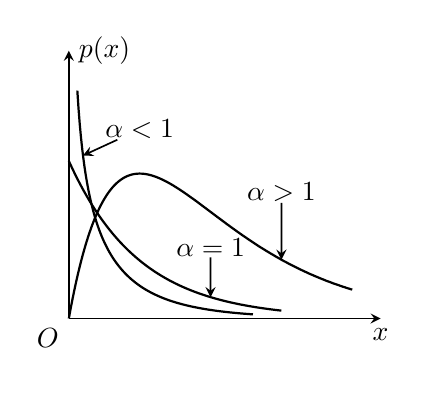
\begin{tikzpicture}[semithick,>=stealth,samples=150,yscale=2,xscale=0.9]
            \draw[->](0,0)node[below left]{$O$}--(4.4,0)node[below]{$x$};
            \draw[->](0,0)--(0,1.7)node[right]{$p(x)$};
            \draw[thick,domain=0.12:2.6]plot(\x,{e^(-\x)/sqrt(\x)/1.77});
            \draw[thick,domain=0:3]plot(\x,{e^(-\x)});
            \draw[thick,domain=0:4]plot(\x,{2.5*(\x)*e^(-\x)});
            \node[inner sep=0pt](a)at(2,0.45){$\alpha=1$};
            \node[inner sep=0pt](b)at(1,1.2){$\alpha<1$};
            \node[inner sep=0pt](c)at(3,0.8){$\alpha>1$};
            \draw[->](a)--(2,{e^(-2)});
            \draw[->](b)--(0.2,{e^(-0.2)/sqrt(0.2)/1.77});
            \draw[->](c)--(3,{2.5*(3)*e^(-3)});
            \node[below]at(1,0){\phantom{$\frac{\alpha-1}\lambda$}};
        \end{tikzpicture}
    }
    \subfloat{
        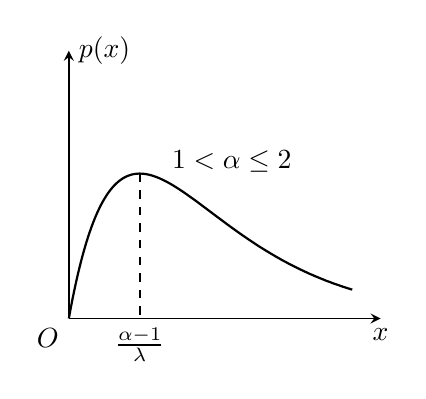
\begin{tikzpicture}[semithick,>=stealth,samples=150,yscale=2,xscale=0.9]
            \draw[->](0,0)node[below left]{$O$}--(4.4,0)node[below]{$x$};
            \draw[->](0,0)--(0,1.7)node[right]{$p(x)$};
            \draw[thick,domain=0:4]plot(\x,{2.5*(\x)*e^(-\x)});
            \draw[dashed](1,{2.5*e^(-1)})--(1,0)node[below]{$\frac{\alpha-1}\lambda$};
            \node at(2.3,1){$1<\alpha\leq2$};
        \end{tikzpicture}
    }
    \subfloat{
        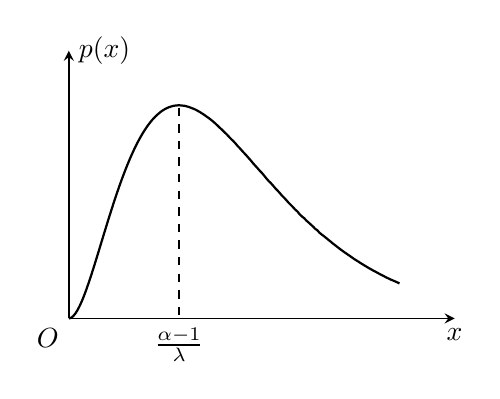
\begin{tikzpicture}[semithick,>=stealth,samples=150,yscale=2,xscale=0.7]
            \draw[->](0,0)node[below left]{$O$}--(7,0)node[below]{$x$};
            \draw[->](0,0)--(0,1.7)node[right]{$p(x)$};
            \draw[thick,domain=0:6]plot(\x,{2.5*(\x)^2*e^(-\x)});
            \draw[dashed](2,{1.5*2^2*e^(-1.5)})--(2,0)node[below]{$\frac{\alpha-1}\lambda$};
        \end{tikzpicture}
    }
    \caption{$\lambda$固定、不同$\alpha$的伽玛密度曲线}\label{fig2.5.5}
\end{figure}

Gamma分布的特征:
\begin{description}
    \item[矩母函数] $M(t)=(\frac{\lambda}{\lambda-t})^{\alpha} , \quad t<\lambda$
    \item[均值] $\mu=\frac{\alpha}{\lambda}$
    \item[方差] $\sigma^2=\frac{\alpha}{\lambda^{2}}$
\end{description}

Gamma函数$\Gamma(\alpha)=\int_0^{\infty}y^{\alpha-1}\ee^{-y}dy$的特征:
\begin{itemize}
    \item $\Gamma(1)=1$
    \item $\Gamma(\frac{1}{2})=\sqrt{\pi}$
    \item $\Gamma(\alpha)=(\alpha-1)\Gamma(\alpha-1)$
    \item $\Gamma(n)=(n-1)!,\quad n \in \mathbb{Z}$
    \item $\Gamma(\frac{\alpha}{2})=\frac{\sqrt{\pi}(\alpha-1)!}{2^{\alpha-1}(\frac{\alpha-1}{2})!}, \quad \alpha=2k+1,k \in \mathbb{N}$
\end{itemize}

\begin{proposition}\label{prop:sum_of_Gamma}
    $\Gamma$分布是指数分布的泛化,即$\Gamma(1,\lambda)=E(\lambda)$。进一步有:若随机变量$X_1,\cdots ,X_k, \operatorname{i.i.d.} \sim E(\lambda)$,则$Y=X_1+\cdots+X_k  \sim \Gamma(k,\lambda)$。更进一步有:若随机变量$X_1',\cdots ,X_k', \operatorname{i.i.d.} \sim \Gamma(\alpha_i,\lambda)$,则$Y'=X_1'+\cdots+X_k'  \sim \Gamma(\alpha_1+\cdots +\alpha_k,\lambda)$。
\end{proposition}

\begin{proof}
    \begin{align*}
        M_Y(t)    & =\prod_{i=1}^k M_{X_i}(t_i)=\prod_{i=1}^k \frac{\lambda}{\lambda-t}=(\frac{\lambda}{\lambda-t})^{k}                                       \\
        M_{Y'}(t) & =\prod_{i=1}^k M_{X_i'}(t_i)=\prod_{i=1}^k (\frac{\lambda}{\lambda-t})^{\alpha_i}=(\frac{\lambda}{\lambda-t})^{\alpha_1+\cdots +\alpha_k}
    \end{align*}
\end{proof}

\begin{proposition}
    若令随机变量$X \sim \Gamma(\alpha,\lambda)$,则$cX \sim \Gamma(\alpha,\frac{\lambda}{c}), \quad c>0$
\end{proposition}

\begin{proof}
    \[ M_{c X}(t) = M_X(c t) =(\frac{\lambda}{\lambda-c t})^{\alpha}=(\frac{\frac{\lambda}{c}}{\frac{\lambda}{c}-t})^{\alpha}\]
\end{proof}

\begin{proposition}
    若令随机变量$X \sim \Gamma(\alpha,\lambda)$,则$\mu_k=\frac{\Gamma(\alpha+k)}{\lambda^{k}\Gamma(\alpha)}, \quad 0<k$,且则$\mu_{-k}=\frac{\lambda^{k}\Gamma(\alpha-k)}{\Gamma(\alpha)}, \quad 0<k<\alpha$
\end{proposition}

\begin{proof}
    \begin{align*}
        \mu_k=M_X^{(k)}(0)     & =\frac{1}{\lambda^{k}}\alpha(\alpha+1)\cdots(\alpha+k-1) =\frac{\Gamma(\alpha+k)}{\lambda^{k}\Gamma(\alpha)} \\
        \mu_{-k}=M_X^{(-k)}(0) & =\lambda^{k}\frac{1}{\alpha-1}\cdots\frac{1}{\alpha-k} =\frac{\lambda^{k}\Gamma(\alpha-k)}{\Gamma(\alpha)}
    \end{align*}
\end{proof}



\begin{proposition}
    %TODO 指数分布、伽马分布与泊松分布间的联系
\end{proposition}

\subsection{贝塔分布}

\begin{definition}
    称以下函数
    \[ \beta(a,b) = \int_0^1 x^{a-1}(1-x)^{b-1}\dd x \]
    为\textbf{贝塔函数},其中参数$a>0,b>0$.
\end{definition}

\begin{proposition}
    贝塔函数具有如下性质:
    \begin{itemize}
        \item $\beta(a,b)=\beta(b,a)$
        \item $\beta(a,b) = \frac{\Gamma(a)\Gamma(b)}{\Gamma(a+b)}$
    \end{itemize}
\end{proposition}

\begin{proof}
    在贝塔函数的积分中令$y=1-x$,即得
    \[ \beta(a,b) = \int_1^0(1-y)^{a-1}y^{b-1}(-\dd y) = \int_0^1 (1-y)^{a-1}y^{b-1}\dd y = \beta(b,a) \]
    由伽玛函数的定义知
    \[ \Gamma(a) \Gamma(b) = \int_0^{+\infty}\int_0^{+\infty}x^{a-1}y^{b-1}  \ee^{-(x+y)} \dd x \dd y \]
    作变量变换$x=uv,y=u(1-v)$,其雅可比行列式$J=-u$,故
    \begin{align*}
        \Gamma(a)\Gamma(b) & = \int_0^{+\infty}\int_0^1(uv)^{a-1}[u(1-v)]^{b-1}
        \ee^{-u}u \dd u \dd v                                                                    \\
                           & = \int_0^{+\infty}u^{a+b-1}\ee^{-u} \int_0^1v^{a-1}(1-v)^{b-1}\dd v
        = \Gamma(a+b)                                                                            \\beta(a,b),
    \end{align*}
\end{proof}

\begin{definition}
    若随机变量$X$的密度函数为
    \[ p(x) = \begin{cases}
            \frac{\Gamma(a+b)}{\Gamma(a)\Gamma(b)}
            x^{a-1}(1-x)^{b-1}, & 0 < x < 1;   \\
            0,                  & \text{其他},
        \end{cases} \]
    则称$X$服从\textbf{贝塔分布},记作$X\sim Be(a,b)$,其中$a>0,b>0$都是形状参数.
\end{definition}

\begin{figure}
    \centering
    \subfloat{
        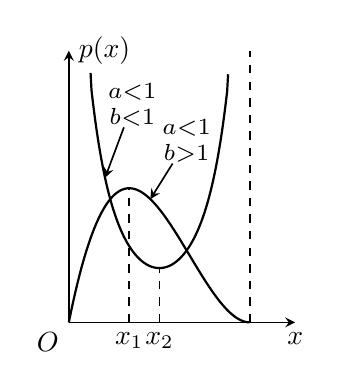
\begin{tikzpicture}[semithick,>=stealth,samples=150,scale=2.3]
            \draw[->](0,0)node[below left]{$O$}--(1.25,0)node[below]{$x$};
            \draw[->](0,0)--(0,1.5)node[right]{$p(x)$};
            \draw[thick,domain=0:1] plot(\x,{5*(\x)*(1-\x)^2});
            \draw[thick,domain=0.12:0.88] plot(\x,{(\x)^(-1/2)*(1-\x)^(-1/2)-1.7});
            \draw[dashed](1,0)--(1,1.5);
            \node[inner sep=0pt](a)at(0.35,1.2){\scalebox{1.2}{$a<1\atop b<1$}};
            \node[inner sep=0pt](b)at(0.65,1){\scalebox{1.2}{$a<1\atop b>1$}};
            \draw[->](a)--(0.2,{(0.2)^(-1/2)*(1-0.2)^(-1/2)-1.7});
            \draw[->](b)--(0.45,{5*(0.45)*(1-0.45)^2});
            \draw[dashed](1/3,0)node[below]{$x_1$}--(1/3,{5*(1/3)*(1-1/3)^2});
            \draw[dashed](0.5,0)node[below]{$x_2$}--(0.5,{(0.5)^(-1/2)*(1-0.5)^(-1/2)-1.7});
        \end{tikzpicture}
    }
    \subfloat{
        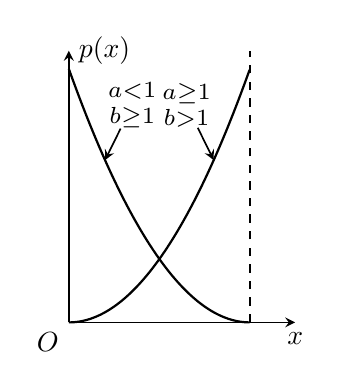
\begin{tikzpicture}[semithick,>=stealth,samples=150,scale=2.3]
            \draw[->](0,0)node[below left]{$O$}--(1.25,0)node[below]{$x$};
            \draw[->](0,0)--(0,1.5)node[right]{$p(x)$};
            \draw[thick,domain=0:1] plot(\x,{1.4*(1-\x)^2});
            \draw[thick,domain=0:1] plot(\x,{1.4*(\x)^2});
            \node[inner sep=0pt](a)at(0.35,1.2){\scalebox{1.2}{$a<1\atop b\geq1$}};
            \node[inner sep=0pt](b)at(0.65,1.2){\scalebox{1.2}{$a\geq1\atop b>1$}};
            \draw[->](a)--(0.2,{1.4*(0.8)^2});
            \draw[->](b)--(0.8,{1.4*0.8^2});
            \draw[dashed](1,0)--(1,1.5);
        \end{tikzpicture}
    }
    \subfloat{
        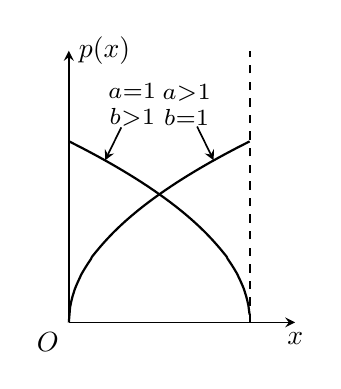
\begin{tikzpicture}[semithick,>=stealth,samples=150,scale=2.3]
            \draw[->](0,0)node[below left]{$O$}--(1.25,0)node[below]{$x$};
            \draw[->](0,0)--(0,1.5)node[right]{$p(x)$};
            \draw[thick,domain=0:1] plot(\x,{1*(1-\x)^(1/2)});
            \draw[thick,domain=0:1] plot(\x,{1*(\x)^(1/2)});
            \node[inner sep=0pt](a)at(0.35,1.2){\scalebox{1.2}{$a=1\atop b>1$}};
            \node[inner sep=0pt](b)at(0.65,1.2){\scalebox{1.2}{$a>1\atop b=1$}};
            \draw[->](a)--(0.2,{1*(0.8)^(1/2)});
            \draw[->](b)--(0.8,{1*0.8^(1/2)});
            \draw[dashed](1,0)--(1,1.5);
        \end{tikzpicture}
    }
    \subfloat{
        \begin{tikzpicture}[semithick,>=stealth,samples=150,scale=2.3]
            \draw[->](0,0)node[below left]{$O$}--(1.25,0)node[below]{$x$};
            \draw[->](0,0)--(0,1.5)node[right]{$p(x)$};
            \draw[thick](0,0.7)--(1,0.7);
            \draw[dashed](1,0)node[below]{$1$}--(1,0.7);
            \node[inner sep=0pt](a)at(0.6,1){\scalebox{1.2}{$a=1\atop b=1$}};
            \draw[->](a)--(0.3,0.7);
        \end{tikzpicture}
    }
    \caption{贝塔密度函数曲线}\label{fig2.5.6}
\end{figure}

从图 \ref{fig2.5.6} 可以看出:
\begin{itemize}
    \item $a<1,b<1$时,$p(x)$是下凸的单峰函数.
    \item $a>1,b>1$时,$p(x)$是上凸的单峰函数.
    \item $a<10,b\ge1$时,$p(x)$是下凸的单调减函数.
    \item $a\ge1,b<1$时,$p(x)$是下凸的单调增函数.
    \item $a=1,b=1$时,$p(x)$是常函数,且$Be(1,1)=U(0,1)$.
\end{itemize}

Beta分布的特征:
\begin{description}
    \item[矩母函数] $M(t)=1+\sum_{k=1}^{\infty}(\prod_{r=0}^{k-1} \frac{a+r}{a+b+r})\frac{t^k}{k!}, \quad t<\lambda$
    \item[均值] $\mu=\frac{a}{a+b}$
    \item[方差] $\sigma^2=\frac{ab}{(a+b+1)(a+b)^{2}}$
\end{description}

\begin{remark}
    \[ \beta(1,1)=U(0,1) \]
\end{remark}

\begin{proposition}
    令独立随机变量$X_1 \sim \Gamma(\alpha_1,\lambda),X_2 \sim  \Gamma(\alpha_2,\lambda)$,则$\frac{X_1}{X_1+X_2} \sim \beta(\alpha_1,\alpha_2)$
\end{proposition}

\begin{proof}
    %TODO 李P182习题38
\end{proof}

\section{正态分布及其导出分布}

\subsection{正态分布}

\begin{definition}
    若随机变量$X$的密度函数为
    \begin{equation}\label{eq2.5.1}
        p(x) = \frac1{\sqrt{2\pi}\sigma} \ee^{-\frac{(x-\mu)^2}{2\sigma^2}},x \in \mathbb{R}
    \end{equation}
    则称$X$服从\textbf{正态分布}(Normal distribution),称$X$为\textbf{正态变量},记作$X\sim N(\mu,\sigma^2)$。其中参数$\mu \in \mathbb{R},\sigma>0$。
\end{definition}

正态分布的密度函数$p(x)$的图形如图 \ref{fig2.5.1}(a)所示,是一条钟形曲线,左右关于$\mu$对称,衰减速度由$\sigma$决定,$\mu\pm\sigma$是该曲线的拐点.

\begin{figure}[!ht]
    \centering
    \subfloat[密度函数$p(x)$]{
        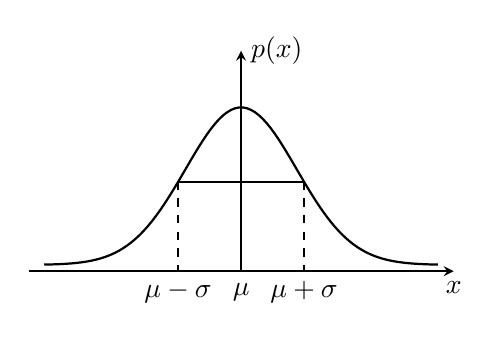
\begin{tikzpicture}[semithick,yscale=2,>=stealth]
            \draw[->](-2.7,0)--(0,0)node[below=1pt]{$\mu$}--(2.7,0)node[below]{$x$};
            \draw[->](0,0)--(0,1.4)node[right]{$p(x)$};
            \draw[samples=100,domain=-2.5:2.5,thick]plot(\x,{e^(-(\x)^2)+0.04});
            \draw[dashed](-0.8,{e^(-0.64)+0.04})--(-0.8,0)node[below]{$\mu-\sigma$}
            (0.8,{e^(-0.64)+0.04})--(0.8,0)node[below]{$\mu+\sigma$};
            \draw(0.8,{e^(-0.64)+0.04})--(-0.8,{e^(-0.64)+0.04});
        \end{tikzpicture}
    }\hspace{1.5cm}
    \subfloat[分布函数$F(x)$]{
        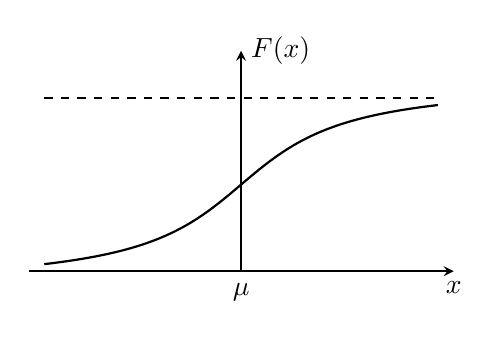
\begin{tikzpicture}[semithick,yscale=2,>=stealth]
            \draw[->](-2.7,0)--(0,0)node[below=1pt]{$\mu$}--(2.7,0)node[below]{$x$};
            \draw[->](0,0)--(0,1.4)node[right]{$F(x)$};
            \draw[samples=100,domain=-2.5:2.5,thick]plot(\x,{(atan(\x))/135+0.55});
            \draw[dashed](-2.5,1.1)--(2.5,1.1);
        \end{tikzpicture}
    }
    \caption{正态分布}\label{fig2.5.1}
\end{figure}

正态分布的特征:
\begin{description}
    \item[矩母函数] $M(t)=\exp (\mu t + \frac{\sigma^2 t^2}{2}), \quad t \in \mathbb{R}$
    \item[均值] $\mu=\mu$
    \item[方差] $\sigma^2=\sigma^2$
\end{description}

\begin{proposition}
    若随机变量$X \sim N(\mu, \sigma^2)$,则其线性变换$a,b \in \mathbb{R},aX + b \sim N(a \mu + b,a^2 \sigma^2)$。特别的,常对正态随机变量作标准化:$\frac{X-\mu}{\sigma} \sim N(0,1)$
\end{proposition}

\begin{proof}
    \[ M_{aX + b}(t)=e^{bt}M_X(a t)=\exp (bt + a \mu t+\frac{a^2 \sigma^2 t^2}{2}) \]
\end{proof}

\begin{proposition}
    若独立随机变量$X_1,\cdots ,X_k$满足$ X_i \sim N(\mu_i,\sigma_i^2)$,则其和$Y=X_1+\cdots +X_k \sim N(\sum_{i=1}^k\mu_i,\sum_{i=1}^k\sigma_i^2)$
\end{proposition}

\begin{proof}
    \[ M_{X_1+\cdots+ X_n} = \prod_{i=1}^n M_{X_i}(t)=\exp (\sum_{i=1}^k\mu_i t + \sum_{i=1}^k \frac{\sigma_i^2 t^2}{2}) \]
\end{proof}

\begin{corollary}
    若随机变量$X_1,\cdots ,X_k \operatorname{i.i.d.} \sim N(\mu,\sigma^2)$,则其平均$\overline{X}=(X_1+\cdots +X_k)/k \sim N(\mu,\frac{\sigma^2}{k})$
\end{corollary}

\begin{theorem}\label{thm:normal_sample_mean_variance}
    若随机变量$X_1,\cdots ,X_k \operatorname{i.i.d} \sim N(\mu,\sigma^2)$,并且定义其样本均值为$\overline{X_n}=\frac{1}{n}\sum_{i=1}^n X_i$,其样本方差为$S_n^2=\frac{1}{n-1}\sum_{i=1}^n (X_i-\overline{X_n})^2$,则有以下关系:
    \begin{enumerate}
        \item $\overline{X_n} \sim N(\mu,\frac{\sigma^2}{n})$,即$\sqrt{n}(\overline{X_n}-\mu)/\sigma \sim N(0,1)$
        \item 随机变量$\overline{X_n}$与随机向量$(X_1-\overline{X_n},\cdots ,X_n-\overline{X_n})$独立
        \item $\overline{X_n},S_n^2$独立
        \item $\frac{(n-1)S_n^2}{\sigma} \sim \chi_n$
        \item $\frac{\sqrt{n}(\overline{X_n}-\mu)}{S_n} \sim t_{n-1}$
    \end{enumerate}
\end{theorem}
\begin{proof}
    %TODO
\end{proof}

\subsection{卡方分布}

\begin{definition}
    设$Z_1,\dotsc,Z_n$独立同分布于标准正态分布$N(0,1)$,则$X=Z_1^2+\dotsc+Z_n^2$的分布称为\textbf{$n$自由度}的\textbf{卡方分布}(Chi-square distribution),记为$X \sim \chi^2_n$.
\end{definition}

卡方分布的特征:
\begin{description}
    \item[参数] $n \in \mathbb{N}_+$
    \item[概率密度函数] $p(x)=\begin{cases}
                \frac{(1/2)^{\frac n2}}{\Gamma(n/2)}y^{\frac n2-1}\ee^{-\frac y2} & y>0         \\
                0                                                                 & \text{其他}
            \end{cases}$
    \item[矩母函数] $M(t)=(\frac{1}{1-2t})^{\frac{n}{2}}$
    \item[均值] $\mu=n$
    \item[方差] $\sigma^2=2n$
    \item[实例]
\end{description}

该密度函数的图像是一个只取非负值的偏态分布,见图~\ref{fig:5.4.1}。
\begin{figure}[!ht]
    \centering
    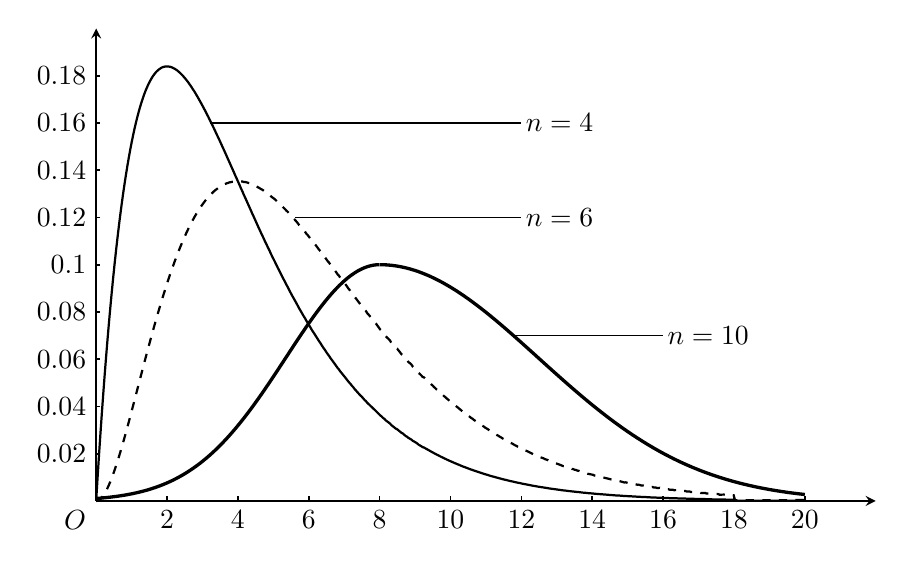
\begin{tikzpicture}[>=stealth,semithick,xscale=0.45,yscale=30,samples=500]
        \draw[->](0,0)node[below left]{$O$}--(22,0);
        \foreach\x in{2,4,...,20}\draw(\x,0.002)--(\x,0)node[below]{\x};
        \draw[->](0,0)--(0,0.2);
        \foreach\x in{0.02,0.04,0.06,0.08,0.1,0.12,0.14,0.16,0.18}\draw(0,\x)node[left]{\x}--(0.12,\x);
        \draw[thick,domain=0:20]plot(\x,{(\x)*e^(-(\x)/2)/4});
        \draw(3.2,0.16)--(12,0.16)node[right=-2pt]{$n=4$};
        \draw[thick,dashed,domain=0:20]plot(\x,{(\x)^2*e^(-(\x)/2)/16});
        \draw[very thick,domain=0:8]plot(\x,{0.1*e^(-(\x-8)^2/14)});
        \draw[very thick,domain=8:20]plot(\x,{0.1*e^(-(\x-8)^2/40)});
        \draw(5.62,0.12)--(12,0.12)node[right=-2pt]{$n=6$};
        \draw(11.8,0.07)--(16,0.07)node[right=-2pt]{$n=10$};
    \end{tikzpicture}
    \caption{$\chi^2(n)$分布的密度函数}\label{fig:5.4.1}
\end{figure}

\begin{proposition}
    若 $X\sim N(0,1)$,则$X^2\sim Ga(1/2,1/2),Y \sim Ga(n/2,1/2)=\chi^2(n)$
\end{proposition}

\begin{proof}
    %TODO \ref{prop:sum_of_Gamma}
\end{proof}

\begin{corollary}
    若随机变量$X_1,\cdots ,X_k, \operatorname{i.i.d.} \sim \chi^2_{n_i}$,则$Y=X_1+\cdots+X_k  \sim \chi^2_{n_1+\cdots +n_k}$。
\end{corollary}

\subsection{F分布}

\begin{definition}{}{}
    设独立随机变量$X_1\sim\chi^2(m),X_2\sim\chi^2(n)$,则称$F=\frac{X_1/m}{X_2/n}$的分布是自由度为$m$与$n$的\textbf{F分布},记为$F\sim F(m,n)$,其中$m$称为\underline{分子自由度},$n$称为\underline{分母自由度}。
\end{definition}

F分布的特征:
\begin{description}
    \item[参数] $m,n \in \mathbb{N}_+$
    \item[概率密度函数]
        \[ f(x)=\frac{\Gamma \left( \frac{m+n}{2} \right) }{\Gamma \left( \frac{m}{2} \right) \Gamma \left( \frac{n}{2} \right)}\left( \frac{m}{n} \right) ^{\frac{m}{2}}x^{\frac{m}{2}-1}\left( 1+\frac{m}{n}x \right) ^{-\frac{m+n}{2}} \]
    \item[矩母函数] 不存在
    \item[均值] $\mu=\frac{n}{n-2}$
    \item[方差] $\sigma^2=\frac{2n^2(m+n-2)}{m(n-2)^2(n-4)}$
    \item[实例]
\end{description}

\begin{figure}
    \centering
    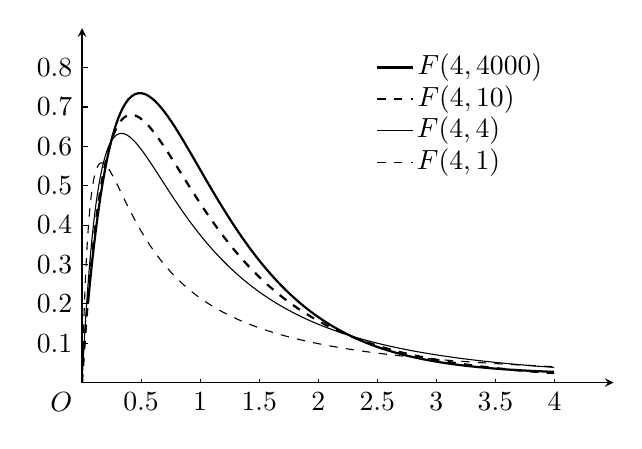
\begin{tikzpicture}[xscale=1.5,yscale=5,>=stealth,domain=0:4,samples=500]
        \draw[->](0,0)node[below left]{$O$}--(4.5,0);\draw[->](0,0)--(0,0.9);
        \foreach \x in{0.5,1,...,4}\draw(\x,0.01)--(\x,0)node[below]{$\x$};
        \foreach \x in{0.1,0.2,0.3,0.4,0.5,0.6,0.7,0.8}\draw(0.05,\x)--(0,\x)node[left]{$\x$};
        \draw[dashed]plot (\x,{12*(\x)/(1+4*(\x))^(5/2)});
        \draw plot (\x,{6*(\x)/(1+\x)^4});
        \draw[thick,dashed]plot (\x,{4.8*(\x)/(1+0.4*(\x))^7});
        \draw[thick,domain=0.05:4]plot (\x,{4*(\x)/(1+0.04*\x)^52+0.02});
        \draw[thick](2.5,.8)--(2.8,.8)node[right=-2pt]{$F(4,4000)$};
        \draw[thick,dashed](2.5,.72)--(2.8,.72)node[right=-2pt]{$F(4,10)$};
        \draw(2.5,.64)--(2.8,.64)node[right=-2pt]{$F(4,4)$};
        \draw[dashed](2.5,.56)--(2.8,.56)node[right=-2pt]{$F(4,1)$};
    \end{tikzpicture}
    \caption{$F$分布的密度函数,是一个只取非负值的偏态分布}\label{fig:5.4.2}
\end{figure}

\begin{proposition}
    $F$分布的密度函数为
\end{proposition}

\begin{proof}
    首先我们导出$Z=\frac{X_1}{X_2}$的密度函数,若记$p_1(x)$和$p_2(x)$分别为$\chi^2(m)$和$\chi^2(n)$的密度函数,根据独立随机变量商的分布的密度函数公式\ref{equ:quotient_of_variable}。$Z$的密度函数为
    \begin{align*}
        p_Z(z) & =\int_0^{=\infty}x_2p_1(zx_2)p_2(x_2)\dd x_2                                                                                                                                       \\
               & =\frac{z^{\frac{m}{2}-1}}{\Gamma \left( \frac{m}{2} \right) \Gamma \left( \frac{n}{2} \right) 2^{\frac{m+n}{2}}}\int_0^{+\infty}x_2^{\frac{m+n}2-1}\ee^{-\frac{x_2}2(1+z)}\dd x_2.
    \end{align*}
    运用变换$u=\frac{x_2}2(1+z)$,可得
    \[p_Z(z)=\frac{z^{\frac{m}{2}-1}\left( 1+z \right) ^{\frac{m+n}{2}}}{\Gamma \left( \frac{m}{2} \right) \Gamma \left( \frac{n}{2} \right)}\int_0^{+\infty}u^{\frac{m+n}2-1}\ee^{-u}\dd u.\]
    最后的定积分为伽马函数$\Gamma\left(\frac{m+n}2\right)$,从而
    \[
        p_Z\left( z \right) =\frac{\Gamma \left( \frac{m+n}{2} \right)}{\Gamma \left( \frac{m}{2} \right) \Gamma \left( \frac{n}{2} \right)}z^{\frac{m}{2}-1}\left( 1+z \right) ^{-\frac{m+n}{2}},\quad z>0.
    \]
    第二步,我们导出$F=\frac nm Z$的密度函数,对$y>0$,有
    \begin{align*}
        p_F\left( y \right) & =p_Z\left( \frac{m}{n}y \right) \cdot \frac{m}{n}                                                                                                                                                                            \\
                            & =\frac{\Gamma \left( \frac{m+n}{2} \right)}{\Gamma \left( \frac{m}{2} \right) \Gamma \left( \frac{n}{2} \right)}\left( \frac{m}{n}y \right) ^{\frac{m}{2}-1}\left( 1+\frac{m}{n}y \right) ^{-\frac{m+n}{2}}\cdot \frac{m}{n} \\
                            & =\frac{\Gamma \left( \frac{m+n}{2} \right) \left( \frac{m}{n} \right) ^{\frac{m}{2}}}{\Gamma \left( \frac{m}{2} \right) \Gamma \left( \frac{n}{2} \right)}y^{\frac{m}{2}-1}\left( 1+\frac{m}{n}y \right) ^{-\frac{m+n}{2}}.
    \end{align*}
\end{proof}

\begin{remark}
    由$F$分布的构造知,若$F\sim F(m,n)$,则有$1/F\sim F(n,m)$
\end{remark}

\subsection{t分布}

\begin{definition}
    设随机变量$Z \sim N(0,1)$与$U \sim\chi^2_n$独立,则称$t=\frac{Z}{\sqrt{U/n}}$的分布为自由度为$n$的\textbf{t分布},记为$t \sim t_n$.
\end{definition}

$t$分布的密度函数的图像是一个关于纵轴对称的分布(图~\ref{fig:5.4.3} ),与标准正态分布的密度函数形状类似,只是峰比标准正态分布低一些,尾部的概率比标准正态分布的大一些.
\begin{figure}
    \centering
    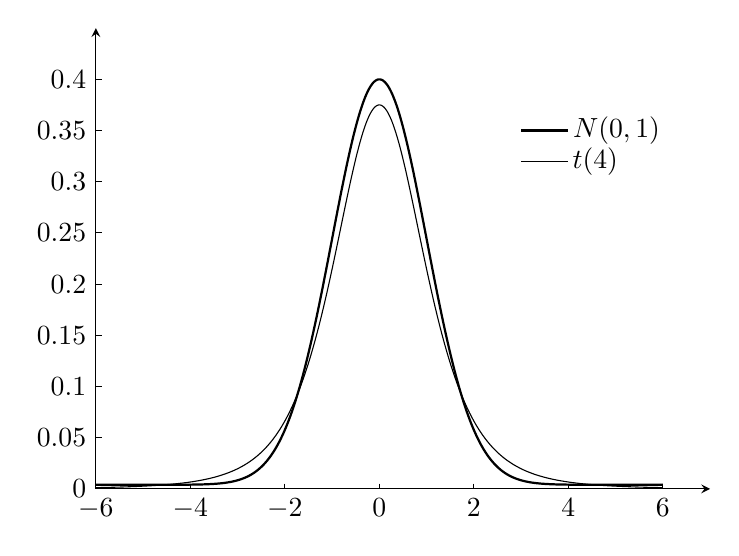
\begin{tikzpicture}[xscale=0.6,yscale=13,>=stealth,domain=-6:6,samples=500]
        \draw[->](-6,0)--(7,0);\draw[->](-6,0)--(-6,0.45);
        \foreach \x in{-6,-4,...,6}\draw(\x,0.005)--(\x,0)node[below]{$\x$};
        \foreach \x in{0,0.05,0.1,0.15,0.2,0.25,0.3,0.35,0.4}\draw(-5.88,\x)--(-6,\x)node[left]{$\x$};
        \draw[thick]plot(\x,{0.396*e^(-(\x)^2/2)+0.004});
        \draw plot(\x,{0.375*(1+(\x)^2/4)^(-5/2)});
        \draw[thick](3,0.35)--(4,0.35)node[right=-2pt]{$N(0,1)$};
        \draw(3,0.32)--(4,0.32)node[right=-2pt]{$t(4)$};
    \end{tikzpicture}
    \caption{$t$分布与$N(0,1)$的密度函数,t分布尾更重}\label{fig:5.4.3}
\end{figure}

t分布的特征:
\begin{description}
    \item[参数] $n \in \mathbb{N}_+$
    \item[概率密度函数] $p(x)=\frac{\Gamma \left( \frac{n+1}{2} \right)}{\sqrt{n\pi}\Gamma \left( \frac{n}{2} \right)}\left( 1+\frac{y^2}{n} \right) ^{-\frac{n+1}{2}}$
    \item[矩母函数] 不存在
    \item[均值] $\mu=0, n>1$
    \item[方差] $\sigma^2=\frac{n}{n-2}, n>2$
    \item[实例]
\end{description}

\begin{remark}
    \begin{itemize}
        \item 自由度$n=1$的t分布就是标准柯西分布,它的均值不存在;
        \item 自由度$n\to \infty$时,$t_n$趋近于$N(0,1)$
    \end{itemize}
\end{remark}

\begin{proposition}
    t分布的密度函数为
\end{proposition}

\begin{proof}
    由标准正态密度函数的对称性知, $X_1$与$-X_1$有相同分布,从而$t$与$-t$有相同分布.这意味着: 对任意实数$y$有
    \[P(0<t<y)=P(-y<-t<y)=P(-y<-t<0).\]

    于是
    \[P(0<t<y)=\frac12P(t^2<y^2).\]

    由$F$变量构造可知, $t^2=\frac{X_1^2}{X_2^2/n}\sim F(1,n)$,将上式两边关于$y$求导可微$t$分布的密度函数为
    \begin{align*}
        p_t(y) & =yp_F(y^2)=\frac{\Gamma \left( \frac{1+n}{2} \right) \left( \frac{1}{n} \right) ^{\frac{1}{n}}}{\Gamma \left( \frac{1}{2} \right) \Gamma \left( \frac{n}{2} \right)}\left( y^2 \right) ^{\frac{1}{2}-1}\left( 1+\frac{1}{n}y^2 \right) ^{-\frac{1+n}{2}}y \\
               & =\frac{\Gamma \left( \frac{n+1}{2} \right)}{\sqrt{n\pi}\Gamma \left( \frac{n}{2} \right)}\left( 1+\frac{y^2}{n} \right) ^{-\frac{n+1}{2}},\quad -\infty<y<+\infty.
    \end{align*}
\end{proof}

\subsection{柯西分布}

\begin{definition}
    若随机变量$X$的密度函数为
    \[ f(x) = \frac{\sigma}{\pi} \frac1{\sigma^2+(x-\mu)^2} ,x \in \mathbb{R} \]
    则称$X$服从\textbf{柯西分布}(Cauchy distribution),记作$X\sim C(\mu,\sigma)$。其中参数$\mu \in \mathbb{R},\sigma>0$。
\end{definition}

\begin{figure}[ht]
    \centering
    \subfloat[柯西分布累积函数]{
        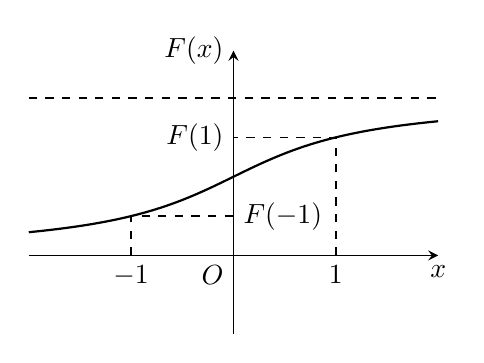
\begin{tikzpicture}[>=stealth,xscale=1.3,yscale=2,semithick]
            \draw[->](-2,0)--(0,0)node[below left]{$O$}--(2,0)node[below]{$x$};
            \draw[->](0,-0.5)--(0,1.3)node[left]{$F(x)$};
            \draw[dashed](-2,1)--(2,1)(1,0)node[below]{$1$}--(1,0.75)--(0,0.75)node[left]{$F(1)$}
            (-1,0)node[below]{$-1$}--(-1,0.25)--(0,0.25)node[right]{$F(-1)$};
            \draw[thick,domain=-2:2,samples=100]plot(\x,{(atan(\x))/180+0.5});
        \end{tikzpicture}
    }
    \subfloat[柯西分布密度函数]{
        \begin{tikzpicture}
            \begin{axis}[
                    axis lines = middle,
                    xlabel=$x$,
                    ylabel={$f(x)$}
                ]
                \addplot[
                    domain=-10:10,
                    samples=100,
                ]
                {1/pi/(1+x^2)};
            \end{axis}
        \end{tikzpicture}
    }
    \caption{柯西分布}
\end{figure}

柯西分布的特征:
\begin{description}
    \item[累积函数] $F(x)=\frac{1}{2}+\frac{1}{\pi} \arctan(\mu +\sigma x)$
    \item[矩母函数] 除$t=0$外不存在
    \item[特征函数] $\phi_X(t)=\exp (i \mu t - \sigma |t|)$
    \item[均值] 不存在
    \item[方差] 不存在
\end{description}

\begin{remark}
    此类因极端值概率密度较高而导致均值、方差不存在的分布称为重尾分布。
\end{remark}

\begin{figure*}
    \centering
    \includegraphics{image/Cauchy_dist.png}
\end{figure*}

\begin{proposition}
    $C(0,1)=t_1$
\end{proposition}

\begin{proposition}
    若随机变量$X,Y \operatorname{i.i.d.} \sim N(0,1)$,则$\frac{X}{Y} \sim C(0,1)$
\end{proposition}

\begin{proof}
    %TODO
\end{proof}

\begin{proposition}
    若随机变量$X \sim C(\mu, \sigma)$,则其线性变换$a,b \in \mathbb{R},aX + b \sim C(a \mu + b,|a| \sigma)$。
\end{proposition}

\begin{proof}
    \[ \phi_{aX + b}(t)=e^{ibt}\phi_X(a t)=\exp (ibt + ia\mu t-\sigma|a t|) \]
\end{proof}

\begin{proposition}
    若独立随机变量$X_1,\cdots ,X_k$满足$ X_i \sim C(\mu_i,\sigma_i)$,则其和$Y=X_1+\cdots +X_k \sim N(\sum_{i=1}^k\mu_i,\sum_{i=1}^k\sigma_i)$
\end{proposition}

\begin{proof}
    \[ \phi_{X_1+\cdots+ X_n} = \prod_{i=1}^n \phi_{X_i}(t)=\exp (it\sum_{i=1}^k\mu_i - |t|\sum_{i=1}^k \sigma_i) \]
\end{proof}

\begin{corollary}
    若随机变量$X_1,\cdots ,X_k \operatorname{i.i.d.} \sim N(\mu,\sigma^2)$,则其平均$\overline{X}=(X_1+\cdots +X_k)/k \sim C(\mu,\sigma)$
\end{corollary}

\begin{remark}
    此处的$\sigma$不代表方差,所以不遵守$\operatorname{Var}(\overline{X})=\frac{\sigma^2}{k}$的关系。
\end{remark}

\section{各分布间关系}

\begin{figure*}[hp]
    \centering\includegraphics[width=0.95\textwidth]{image/relationship.png}
\end{figure*}

\begin{figure}[hp]
    \centering\includegraphics[width=0.95\textwidth]{image/Relationships_among_some_of_univariate_probability_distributions.jpg}
    \caption{各分布间的联系}
    \label{fig:relationship_among_univariate_distributions}
\end{figure}

可参考网站\url{http://www.math.wm.edu/~leemis/chart/UDR/UDR.html}
\chapter{概率极限}\label{chap:limitation}
\begin{introduction}[考试重点]
    \item 收敛性
    \item Borel-Cantelli引理
    \item 各种概率不等式
    \item 特征函数在处理概率极限定理中的应用
    \item 各种大数定律及证明
    \item 中心极限定理
\end{introduction}
\section{收敛}

\subsection{几乎必然收敛}

\begin{definition}[几乎必然收敛]
    若随机变量序列$\{ X_n: \Omega \to \mathbb{R} \}$与随机变量$X:\Omega \to \mathbb{R}$间存在以下关系:
    \[ \P\{ \omega \in \Omega: \lim_{n \to \infty}\abs{ X_n(\omega) - X(\omega)} < \e \} =1,\quad \forall \e > 0\]
    则称$X_n$\textbf{几乎必然收敛}(converges almost surely)于$X$, 记为$X_n \xrightarrow{\as} X$。
\end{definition}
\begin{remark}
    类似于微积分中逐点收敛的条件。考察满足条件$\lim_{n \to \infty}\abs{ X_n(\omega) - X(\omega)} < \e$的样本点,这些样本点组成事件(可简记为$\{ \lim_{n \to \infty} X_n=X \}$)的概率为$1$。
\end{remark}

\begin{proposition}
    几乎必然收敛的极限几乎处处相等。即若$X_n \xrightarrow{\as} X$且$X_n \xrightarrow{\as} X'$,则 
    \[ \P(X=X')=1 \]
\end{proposition}
\begin{proof}
    若对于$\omega \in \Omega$,满足$\lim_{n \to \infty} X_n(\omega)=X(\omega)$与$\lim_{n \to \infty} X_n(\omega)=X'(\omega)$,则有 $X(\omega)=X'(\omega)$。记
    \begin{align*}
        A &= \{ \omega \in \Omega: \lim_{n \to \infty} X_n(\omega)=X(\omega) \}, \\
        B &= \{ \omega \in \Omega: \lim_{n \to \infty} X_n(\omega)=X'(\omega) \}
    \end{align*}
    则
    \[ A \cap B \in \{ X=X' \} \]
    故
    \[ \P(X=X') \ge \P(A \cap B) = \P(A) + \P(B) - \P(A \cup B) \ge 1 \]
    所以 $\P(X=X')=1$
\end{proof}

\subsection{依概率收敛}

\begin{definition}[依概率收敛]
    若随机变量序列$\{ X_n: \Omega \to \mathbb{R} \}$与随机变量$X:\Omega \to \mathbb{R}$间存在以下关系:
    \[ \lim_{n\to\infty}\P\{\omega \in \Omega: \abs{X_n(\omega) - X(\omega)}<\e\} = 1, \quad \forall \e>0. \]
    则称$X_n$\textbf{依概率收敛}(converges in probability)于$X$, 记为$X_n \xrightarrow{\P} X$。
\end{definition}
\begin{remark}
    即对于事件$A_i=\{\omega \in \Omega: \abs{X_n(\omega) - X(\omega)}<\e\}$,其概率将逐渐变为$1$。
\end{remark}

\begin{figure*}[h]
    \centering
    \includegraphics[width=0.9\textwidth]{image/converge1.png}
\end{figure*}

对于几乎必然收敛的情况,每个样本点上的序列随机变量都在逐渐趋近收敛变量;而对于依概率收敛的情况,由于对某个样本点的概率为0(例如连续随机变量),可能某一次样本点的序列随机变量接近收敛变量,下一次又远离收敛变量,只要保证总体概率趋近$1$即可。

\begin{theorem}[Borel-Cantelli定理]
    在概率空间 $(\Omega,\mathcal{F},\P)$中,设 $\{ A_n \in \mathcal{F} \}$,
    \begin{itemize}
        \item 若 $\sum_{n=1}^{\infty} \P(A_n) < \infty$, 则
        \[ \P(\limsup_{n \to \infty}A_n) = 0\]
        \item 若$\{ A_n \}$是独立事件列,且 $\sum_{n=1}^{\infty} \P(A_n) = \infty$, 则
        \[ \P(\limsup_{n \to \infty}A_n) = 1\]
    \end{itemize}
\end{theorem}

\begin{proposition}
    依概率收敛是几乎必然收敛的\underline{必要条件},但\underline{不是充分条件}。
\end{proposition}

\begin{example}[依概率收敛而不几乎必然收敛]
    设样本空间为$\Omega =(0,1]$,概率均匀分布在样本空间上,即$P([a,b])=b-a,0<a<b<1$。接下来对于$k \in \mathbb{N}_+$,将区间$(0,1]$分为$2^{k}$个等长的子区间,并分别记为$I_{k,j}=(\frac{j-1}{2^k},\frac{j}{2^k}]$。

    按以下方式定义随机变量序列$\{ X_n: \Omega \to \mathbb{R} \}$:
    \[ X_n(\omega)=\begin{cases}
            1, \omega \in I_{k,j}    \\
            0, \omega \notin I_{k,j} \\
        \end{cases} ,\quad n = 2^k+j-2\]
    同时定义随机变量$X: \Omega \to \mathbb{R}$为$X(\omega)=0,\forall \omega \in \Omega$

    由于
    \[ \P\{\omega \in \Omega: \abs{X_n(\omega) - X(\omega)}<\e\}=1-\frac1{2^k} \to 1 ,\quad \forall 0<\epsilon<1 \]
    所以$X_n \xrightarrow{\P} X$。
    然而对于任意$\omega \in \Omega$,无论$k$为何数,此次分割中,总有一个区间包含此样本点。即有无数个$X_i(\omega) = 1$。所以
    \[ \P\{ \omega \in \Omega: \lim_{n \to \infty}\abs{ X_n(\omega) - X(\omega)} < \epsilon \} =\P\{\emptyset \}=0 \]
    所以$X_n$不几乎必然收敛到$X$。
\end{example}

\begin{lemma}\label{lem:sum_product_CP}
    若$X_n \xrightarrow{\P} X, Y_n \xrightarrow{\P} Y$,则:
    \begin{enumerate}
        \item$X_n \pm Y_n \xrightarrow{\P} X \pm Y$
        \item$X_n Y_n \xrightarrow{\P} XY$
    \end{enumerate}
\end{lemma}
\begin{proof}
    \begin{enumerate}
        \item 因为
              \[ \{ \left\vert X_n+Y_n-X-Y \right\vert \ge \e \} \subset \{ \left\vert X_n-X \right\vert \ge \frac{\e}{2} \} \cup \{ \left\vert Y_n-Y \right\vert \ge \frac{\e}{2} \} \]
              所以
              \[ 0 \le P\{ \left\vert X_n+Y_n-X-Y \right\vert \ge \e \} \le P\{ \left\vert X_n-X \right\vert \ge \frac{\e}{2} \} + P\{ \left\vert Y_n-Y \right\vert \ge \frac{\e}{2} \} \]
              对上式取极限,并由夹逼定理得:
              \[ P\{ \left\vert X_n+Y_n-X-Y \right\vert \ge \e \}=0 \]
              由$Y_n \xrightarrow{\P} Y$易得$-Y_n \xrightarrow{\P} -Y$,所以又有$X_n - Y_n \xrightarrow{\P} X - Y$。
        \item 由于$2ab=(a+b)^2-a^2+b^2$,结合上一结论可知:$X_n Y_n \xrightarrow{\P} XY$的充分条件是$X_n \xrightarrow{\P} X \implies X_n^2 \xrightarrow{\P} X^2$。
              任取$\e >0$,有
              \begin{align*}
                  P\{|X_n^2-X^2| \ge \e \}= & P\{|X_n-X||X_n+X| \ge \e \}                         \\
                  =                         & P(\{|X_n-X||X_n+X| \ge \e \} \cap\{|X_n+X| \le M\}) \\
                                            & + P(\{|X_n-X||X_n+X| \ge \e \} \cap \{|X_n+X|>M\})  \\
                  \le                       & P\{|X_n-X| \ge \e / M\}+P\{|X_n+X|>M\}
              \end{align*}
              而
              \begin{align*}
                  P\{|X_n+X|>M\} \le & P\{|X_n-X|+|2X|>M\}                           \\
                  =                  & P(\{|X_n-X|+|2X|>M\} \cap\{|X_n-X|<1\})       \\
                                     & + P(\{|X_n-X|+|2X|>M\} \cap\{|X_n-X| \ge 1\}) \\
                  \le                & P\{|2 X|>M-1\}+P\{|X_n-X| \ge 1\}
              \end{align*}
              将$M$取足够大,使得对于任取的$\delta >0$,有$P\{ |X| >(M-1) / 2 \}< \delta$成立。并且由于$X_n \xrightarrow{\P} X$,所以
              \[ \exists N, \forall n>N \st P\{|X_n-X| \ge \e / M\},P\{|X_n-X| \ge 1\} < \delta \]
              综上
              \begin{align*}
                  P\{|X_n^2-X^2| \ge \e \} & \le P\{|X_n-X| \ge \e / M\}+P\{|X_n+X|>M\}                      \\
                                           & \le P\{|X_n-X| \ge \e / M\} + P\{|2 X|>M-1\}+P\{|X_n-X| \ge 1\} \\
                                           & < 3\delta
              \end{align*}
              即$X_n^2 \xrightarrow{\P} X^2$,所以$X_n Y_n \xrightarrow{\P} XY$
    \end{enumerate}
\end{proof}

\begin{theorem}
    若$X_n \xrightarrow{\P} X$,$g(x)$是$\mathbb{R}$上的连续函数,则$g(X_n) \xrightarrow{\P} g(X)$
\end{theorem}
\begin{proof}
    若$g_m(x)$是$m$次多项式函数,即$g_m(x)=\sum_{i=0}^m a_ix^i$,则由引理\ref{lem:sum_product_CP}知有
    \[ g_m(X_n) \xrightarrow{\P} g_m(X) \]
    因为$g(x)$是连续函数,所以可以用多项式函数去逼近$g(x)$,并且在任意有限区间上还是一致的,即对于任意$M,\e >0$,当$m$足够大的时候,存在$g_m(x)$,满足
    \[ \abs{g(x)-g_m(x)} < \e ,\ \abs x \le M \]

    接下来以$\abs X ,\abs{X_n} \le M$为界,将目标拆为两部分:
    \begin{align*}
            & P\{|g(X_n)-g(X)| \ge \e \}                                                                              \\
        =   & P(\{|g(X_n)-g(X)| \ge \e \}\cap \{\abs X ,\abs{X_n} \le M \})                                           \\
            & +P(\{|g(X_n)-g(X)| \ge \e \}\cap \{\{\abs X \le M\} \cup \{\abs{X_n} \le M\} \})                        \\
        \le & P(\{|g(X_n)-g(X)| \ge \e \}\cap \{\abs X ,\abs{X_n} \le M \}) + P\{\abs X \le M\}+ P\{\abs{X_n} \le M\}
    \end{align*}
    对于后半部分有:
    \[ \forall \delta >0 , \exists M >0 \st P\{\abs X \le M\},P\{\abs{X_n} \le M\}< \delta \]
    对于第一项,将$\{|g(X_n)-g(X)| \ge \e \}$拆分为三部分:
    \[ \{|g(X_n)-g(X)| \ge \e \} \subset \{|g(X_n)-g_m(X_n)| \ge \e / 3 \} \cup \{|g_m(X_n)-g_m(X)| \ge \e / 3 \} \cup \{|g_m(X)-g(X)| \ge \e / 3 \} \]
    又因为多项式函数逼近的一致性,稍加替换可得:
    \begin{align*}
        \left\{|g(X_n)-g_m(X_n)| \ge \e / 3 \right\}\cap\{|X| \le M\} \cap\left\{|X_n| \le M \right\} = & \emptyset \\
        \left\{|g_m(X)-g(X)| \ge \e / 3 \right\}\cap\{|X| \le M\} \cap\left\{|X_n| \le M \right\} =     & \emptyset
    \end{align*}
    所以
    \begin{align*}
            & P(\{|g(X_n)-g(X)| \ge \e \}\cap \{\abs X ,\abs{X_n} \le M \})                                     \\
        \le & P(\left\{|g_m(X_n)-g_m(X)| \ge \e / 3\right\} \cap\{|X| \le M\} \cap\left\{|X_n| \le M+1\right\}) \\
        \le & P\left\{|g_m(X_n)-g_m(X)| \ge \e / 3\right\}<\delta
    \end{align*}
    综上
    \[ P\{|g(X_n)-g(X)| \ge \e \} < 4 \delta\]
    即$g(X_n) \xrightarrow{\P} g(X)$
\end{proof}

\begin{note}
    相关证明技巧总结:对于事件$\{ |X+Y| > a+b \}$,有$\{ |X+Y| > a+b \} \subset \{ |X|>a \} \cup \{ |Y|>b \}$,从而有
    \[ P\{ |X+Y| > a+b \} \le P\{ |X|>a \} + P\{ |Y|>b \} \]
\end{note}

\subsection{依分布收敛}

\begin{definition}[依分布收敛]
    设随机变量$X, X_1, X_2, \dotsc$的分布函数分别为$F(x), F_1(x), F_2(x), \dotsc$。若对$F(x)$的任一\underline{连续点}$x$,都有
    \[ \lim_{n \to +\infty} F_n(x) = F(x) \]
    则称$\{ F_n(x) \}$\textbf{弱收敛}(converge weakly)于$F(x)$, 记作$F_n(x) \xrightarrow{W} F(x)$;也称$\{ X_n \}$\textbf{按分布收敛}(converge in distribution)于$X$,记作$X_n \xrightarrow{d} X$
\end{definition}
\begin{remark}
    对于非连续点,其收敛值可能使得收敛函数不满足分布函数特征(见下例),需要定义这些非连续点上的值,使其满足分布函数特征。
\end{remark}

\begin{example}
    设$\{ X_n \}$服从退化分布:
    \[ P \biggl(X_n = \frac1n \biggr) = 1, \quad n \in N_+\]
    其分布函数分别为:
    \[ F_n(x ) = \begin{cases}
            0, & x < 1/n,    \\
            1, & x \geq 1/n.
        \end{cases} \]
    因为$F_n(x)$是在点$x=1$处有跳跃,所以当$n \to +\infty$时,跳跃点位置趋于0。于是我们很自然地认为$\{ F_n(x) \}$应该收敛于点$x=0$处的退化分布,即
    \[ F(x) = \begin{cases}
            0, & x < 0,    \\
            1, & x \geq 0.
        \end{cases} \]
    但是,对任意的$n$,有$F_n(0) = 0$, 而$F(0) = 1$, 所以
    \[ \lim_{n \to +\infty} F_n(0) = 0 \neq 1 = F(0) \]
\end{example}

\begin{proposition}\label{prop:CP_VS_CD}
    依分布收敛是依概率收敛的\underline{必要条件},但\underline{不是充分条件}。但若依概率收敛到一个\underline{常数随机变量},则也可推出依分布收敛。
\end{proposition}
\begin{remark}
    直观来看,$X_n$依概率收敛到$X$,意味着$n$很大时,二者的距离大概率很近。那么随着$n$越来越大,$X_n$的行为自然会越来越像。对于某一区间$B$,样本点集$X^{-1}(B)=\{\omega\in\Omega : X(\omega) \in B\}$将与点集$X^{-1}_n(B)$越来越接近,其两随机变量出现在此区间的概率也将逐渐相等,这就是依分布收敛描述的东西。
\end{remark}
\begin{proof}
    \textbf{必要性}:设随机变量$X, X_1,  X_2, \dotsc$的分布函数分别为$F(x), F_1(x), F_2(x), \dotsc$。
    \begin{figure}[H]
        \centering
        \begin{subfigure}[]{0.8\textwidth}
            \centering
            \includegraphics[width=\textwidth]{image/CP_to_CF1.jpg}
            \caption{$X_n>X$}
            \label{fig:CP_to_CF1}
        \end{subfigure}
        \begin{subfigure}[]{0.8\textwidth}
            \centering
            \includegraphics[width=\textwidth]{image/CP_to_CF2.jpg}
            \caption{$X_n<X$}
            \label{fig:CP_to_CF2}
        \end{subfigure}
        %\caption{}
        \label{fig:CP_to_CF}
    \end{figure}
    如上图\ref{fig:CP_to_CF1},直观来看$P\{ X_n\le t \} \approx F(t-\e)$。而严格来看有:
    \begin{align*}
        F_n(t) & = P(X_n\le t)                                     \\
               & \ge P(X_n\le t,X\le t-\e)                         \\
               & =P(X\le t-\e) - P(X_n > t,X\le t-\e)              \\
               & \ge F(t-\e) - P(\left\vert X_n-X \right\vert >\e)
    \end{align*}
    数列$\{ F_n(t) \}$的极限未必存在,但可对两边取下极限得
    \[ F(t-\e) \leq \varliminf_{n \to +\infty} F_n(t) \]

    同理,如上图\ref{fig:CP_to_CF2},根据“对称性”,交换$X_n$与$X$的位置有:
    \[ F(t+\e) \ge F_n(t) - P(\left\vert X_n-X \right\vert >\e)\]
    对两边取下极限得
    \[ \varlimsup_{n \to +\infty} F_n(t) \leq  F(t+\e) \]

    综上有:
    \[ F(t-\e) \leq \varliminf_{n \to +\infty} F_n(t) \le \varlimsup_{n \to +\infty} F_n(t) \leq  F(t+\e) \]
    再令$\e \to 0+$得
    \[ F(t-0) \leq \varliminf_{n \to +\infty} F_n(t) \le \varlimsup_{n \to +\infty} F_n(t) \leq  F(t+0) \]
    所以当$t$为$F(x)$上的连续点时,$F(t-0)=F(t+0)$。根据夹逼定理,此时$\{ F_n(t) \}$的极限存在且
    \[ \lim_{n \to +\infty} F_n(x) = F(x) \]

    \textbf{充分性}(常数随机变量):设$X=c$,$c$为常数,其分布函数退化为:
    \[ F(x) = \begin{cases}
            0, & x < c,    \\
            1, & x \geq c.
        \end{cases} \]
    所以对任意的$\e > 0$, 有
    \begin{align*}
        P\{ \left\vert X_n-X \right\vert \ge \e \} & = P\{ X_n \geq c + \e \} + P\{ X_n \le  c - \e \}           \\
                                                   & \leq P\{ X_n > c + \frac{\e}{2} \} + P\{ X_n \le  c - \e \} \\
                                                   & = 1 - F_n(c + \e / 2 ) + F_n(c - \e ).
    \end{align*}
    由于$x = c + \e / 2$和$x = c - \e$均为$F(x)$的连续点,且$F_n(x) \stackrel{W}{\to} F(x)$,所以当$n \to +\infty$时,有
    \[ F_n(c + \e / 2 ) \to F(c + \e / 2 ) = 1, \quad F_n(c - \e) \to F(c - \e ) = 0 \]
    由此得
    \[ P\{ \left\vert X_n-X \right\vert \ge \e \} \to 0 \]
\end{proof}

\begin{example}[依分布收敛而不依概率收敛]
    设$X$的分布列为
    \[ P(X = -1 ) = \frac1{2}, \quad P(X = 1) = \frac1{2} \]
    令$X_n = -X$, 则$X_n$与$X$同分布。即$X_n$与$X$有相同的分布函数。故$X_n \stackrel{L}{\to} X$。

    但对任意$0 < \e < 2$,有
    \[ P\{ \left\vert X_n-X \right\vert \ge \e \} = P(2 \left\vert X \right\vert \geq \e ) = 1 \nrightarrow 0 \]
    即$X_n$不是依概率收敛于$X$。
\end{example}

\begin{figure}[H]
    \centering
    \begin{tikzpicture}
        \node[box](1) at(0,0) {几乎必然收敛};
        \node[box](2) at(4,0) {依概率收敛};
        \node[box](3) at(8,0) {按分布收敛};
        \draw[-to](1)--(2);
        \draw[-to](2)--(3);
        \draw[->,densely dotted](8,0.45) arc(0:180:2);
        \node at(6,1.5) {常数随机变量};
    \end{tikzpicture}
    \caption{三种收敛的关系}
    \label{fig:relationship_among_converges}
\end{figure}

\begin{theorem}[连续映射定理]\label{thm:continuous_mapping}
    设$g: \mathbb{R}^k \mapsto \mathbb{R}$为区间$B$上的\underline{连续}函数,并且$P(X \in B)=1$,则随机向量序列通过次映射后收敛情况与原先相同,即:
    \begin{align*}
        X_n^{(i)} \xrightarrow{\as} X^{(i)}  & \Rightarrow g(X_n^{(1)},\cdots X_n^{(k)}) \xrightarrow{\as} g(X^{(1)},\cdots X^{(k)}) \\
        X_n^{(i)} \xrightarrow{\P} X^{(i)}   & \Rightarrow g(X_n^{(1)},\cdots X_n^{(k)}) \xrightarrow{\P} g(X^{(1)},\cdots X^{(k)})  \\
        (X_n^{(i)}) \xrightarrow{d}(X^{(i)}) & \Rightarrow g(X_n^{(1)},\cdots X_n^{(k)}) \xrightarrow{d} g(X^{(1)},\cdots X^{(k)})   \\
    \end{align*}
\end{theorem}
\begin{proof}
    证明见书\cite[Asymptotic Statistics]{vaart_1998}中定理2.3。
\end{proof}

\begin{corollary}[Slutsky定理]\label{cor:Slutsky}
    若$X_n \xrightarrow{d} X, Y_n \xrightarrow{P} a$,其中$a$是常数,则:
    \begin{itemize}
        \item$Y_n X_n \xrightarrow{d} a X$
        \item$Y_n + X_n \xrightarrow{d} a + X$
        \item$\frac{X_n}{Y_n}  \xrightarrow{d} \frac{X}{a}$,若对所有的$n$都有$P(Y_n\neq 0)=1$,并且$a\neq 0$
    \end{itemize}
\end{corollary}
\begin{proof}
    由条件可知,$(X_n,Y_n) \xrightarrow{d}(X,a)$,且$g_1(X_n,Y_n)=X_n Y_n, g_2(X_n,Y_n)=X_n+Y_n, g_3(X_n,Y_n)=\frac{X_n}{Y_n}$都是连续函数($g_3$在定理中的限制下),所以仍然保持依分布收敛。
\end{proof}
\begin{remark}
    当$Y_n \xrightarrow{P} a$才能得出$(X_n,Y_n) \xrightarrow{d}(X,a)$;若$Y_n$依分布收敛到其他随机变量,则未必成立。
\end{remark}

\begin{theorem}[theta方法的极限定理]
    设
    \[ \frac{\sqrt{n}(X_n-\theta)}{\sigma} \xrightarrow{d} N(0,1) \]
    那么对于连续函数$g$,若$g'(\theta)\neq 0$存在,则
    \[ \frac{\sqrt{n}(g(X_n)-g(\theta))}{\sigma|g'(\theta)|} \xrightarrow{d} N(0,1) \]
\end{theorem}
\begin{proof}
    %TODO
\end{proof}

\begin{theorem}[连续性定理]\label{thm:continuity}
    设$F_n(x)$是一个累计函数序列,并且分别对应矩母函数$M_n(t)$;$F(x)$是一个累计函数,并且对应矩母函数$M(t)$。那么,$F(x)$的所有连续点上$F_n(x) \xrightarrow{M} F(x)$的充要条件是:
    \[ \forall t \in U(0,\delta) ,s.t. \lim_{n \to \infty}M_n(t) = M(t)\]
    其中$U(0,\delta)$代表某一包含零点的开区间。

    若矩母函数不存在,可替换成特征函数
    \[ \forall t \in \mathbb{R} ,\st \lim_{n \to \infty}\varphi_n(t) = \varphi(t)\]
\end{theorem}
\begin{remark}
    不能替换成密度函数或质量函数
\end{remark}

\begin{example}
    \textbf{离散情况}:
    设均匀随机变量$X_n \sim U(-\frac1{2},\frac1{2})$,那么$X_n \xrightarrow{d} 0$。然而$P_n(x) \to 0, \forall x \in \mathbb{R}$(不满足质量函数定义),并且$\lim_{n \to \infty}F_n(0)=\frac1{2}$(不满足累积函数定义)

    \textbf{连续情况}:
    设累积函数为$F_n(x)=x-\frac{\sin(2n\pi x)}{2n\pi}, 0<x<1$,那么$F_n \xrightarrow{d} U(0,1)$。然而$f_n(x)$无极限
\end{example}

\begin{example}[泊松分布收敛于正态分布]
    令$X_n \sim P(\lambda_n)$,并且$\lim_{n \to \infty}\lambda_n =\infty$。将变量标准化:
    \[ Z_n=\frac{X_n-\lambda_n}{\sqrt{\lambda_n}} \]
    那么
    \[M_{Z_n}(t)=\ee^{-t\sqrt{\lambda_n}}M_{X_n}(t)(\frac{t}{\sqrt{\lambda_n}})=\exp(-t\sqrt{\lambda_n}+\lambda_n(e^{\frac{t}{\sqrt{\lambda_n}}-1}))\]
    由于
    \[ \lim_{n \to \infty}\ln(M_{Z_n}(t))=\lim_{\lambda_n \to \infty}-t\sqrt{\lambda_n}+\lambda_n(e^{\frac{t}{\sqrt{\lambda_n}}-1})=\frac{t^2}{2} \]
    所以$Z_n \xrightarrow{d} N(0,1)$,即若$\lambda$很大,可通过$N(\lambda,\lambda)$估计$P(\lambda)$
\end{example}

\section{大数定理}\label{sec:large_number}

大数定律讨论的是在什么条件下,随机变量序列的算术平均依概率收敛到其均值
的算术平均。

\begin{definition}[大数定律的一般形式]\label{def:large_number_law}
    设有一随机变量序列$\{ X_n \}$,若满足:
    \[ \frac1n \sum_{i=1}^n X_i \xrightarrow{\P} \frac1n \sum_{i=1}^n E(X_i) \]
    则称该随机变量序列$\{ X_n \}$服从\textbf{大数定律}。
\end{definition}
\begin{note}
    柯西分布无均值、方差,不存在此定理。
\end{note}

不同的大数定律的差别只是对不同的随机变量序列$\{ X_n \}$而言, 有的是相互独立的随机变量序列, 有的是相依的随机变量序列, 有的是同分布的随机变量序列, 有的是不同分布的随机变量序列等等.

\begin{theorem}[切比雪夫大数定律]
    设$\{ X_n \}$为一列\underline{两两不相关}的随机变量序列,若每个$X_i$的\underline{方差存在,且有共同的上界},即$\Var(X_i) \le c ,\ i=1,2, \dotsc$,则$\{ X_n \}$服从大数定律\ref{def:large_number_law}。
\end{theorem}
\begin{remark}
    切比雪夫大数定律只要求$\{ X_n \}$互不相关, 并不要求它们是同分布的。假如$\{ X_n \}$是独立同分布的随机变量序列, 且方差有限, 则$\{ X_n \}$必定服从大数定律.
\end{remark}
\begin{proof}
    因为$\{ X_n \}$两两不相关,故
    \[ \Var \left(\frac1n \sum_{i=1}^n X_i \right) = \frac1{n^2} \sum_{i=1}^n\Var(X_i) \leq \frac{c}{n} \]
    再由切比雪夫不等式得:
    \[ P \left(\left\lvert \frac1n \sum_{i=1}^n X_i - \frac1n \sum_{i=1}^n E(X_i) \right\rvert \ge  \e \right) < \frac{\Var\left(\frac1n \sum_{i=1}^n X_i \right)}{\e^2} < \frac{c}{n\e^2} ,\quad \forall \e > 0 \]
    于是当$n \to +\infty$时,有
    \[ \lim_{n \to +\infty} P \left(\left\lvert \frac1n \sum_{i=1}^n X_i - \frac1n \sum_{i=1}^n E(X_i) \right\rvert < \e \right) = 1 \]
\end{proof}

\begin{theorem}[马尔可夫大数定律]
    对随机变量序列$\{ X_n \}$,若
    \[ \frac1{n^2}\Var \left(\sum_{i=1}^n X_i \right) \to 0 \]
    成立,则其服从大数定律。此条件被称为\textbf{马尔可夫条件}。
\end{theorem}
\begin{remark}
    马尔可夫条件对$\{ X_n \}$已经没有任何同分布、独立性、不相关的假定。证明过程与切比雪夫大数定律类似;切比雪夫大数定律显然可由马尔可夫大数定律推出。
\end{remark}

\begin{example}\label{ex:4.2.3}
    设$\{ X_n \}$为一同分布、方差存在的随机变量序列,且$X_n$仅与$X_{n-1}$和$X_{n+1}$相关,而与其他的$X_i$不相关。试问该随机变量序列$\{ X_n \}$是否服从大数定律?
\end{example}
\begin{solution}
    考虑其马尔可夫条件
    \[ \frac1{n^2}\Var \left(\sum_{i=1}^n X_i \right) = \frac1{n^2} \left[ \sum_{i=1}^n \Var(X_i) + 2 \sum_{i=1}^{n-1} \Cov(X_i, X_{i-1})\right] \]
    记$\Var(X_i) = \sigma^2$,则$\abs{\Cov(X_i, X_j)}\leq \sigma^2$,于是有
    \[ \frac1{n^2}\Var \left(\sum_{i=1}^n X_i \right) \leq \frac1{n^2} \left[n \sigma^2 + 2(n - 1) \sigma^2\right] \to 0 \]
    即马尔可夫条件成立, 故$\{ X_n \}$服从大数定律.
\end{solution}

\begin{theorem}[(辛钦)弱大数定理]
    设$\{ X_n \}$为一\underline{独立同分布}的随机变量序列,若$X_i$的数学\underline{期望存在}且为$\mu$,则$\{ X_n \}$服从大数定律,即:
    \[ \overline{X_n}=\frac1n\sum_{i=1}^n X_i \xrightarrow{\P} \mu \]
\end{theorem}
\begin{proof}
    因为$\{ X_n \}$同分布,故其特征函数相同,记为$\varphi(t)$。又因为$\varphi'(0)=i \E(X_i)$,则其位于$0$点附近的展开式为:
    \[ \varphi(t)=\varphi(0)+\varphi'(0)t+o(t)=1+i \mu t +o(t) \]
    由$\{ X_n \}$的独立性知$\overline{X_n}$的特征函数为:
    \[ \varphi_{\overline{X_n}}(t)=\left[ \varphi(\frac{t}{n}) \right]^n=\left[ 1+i \mu \frac{t}{n} +o(\frac{t}{n}) \right]^n \]
    对于任意$t$有:
    \[ \lim_{n \to \infty} \varphi_{\overline{X_n}}(t) = \ee^{i \mu t}\]
    再根据定理\ref{thm:continuity}与命题\ref{prop:CP_VS_CD},上述定理成立。
\end{proof}

\begin{example}[蒙特卡洛积分(平均值法)]
    为计算积分$I(f)=\int_0^1 f(x)\mathrm{d}x$,生成随机数$X_1,\cdots ,X_n \operatorname{i.i.d.} \sim U(0,1)$,并且计算$\hat{I}(f)=\overline{Y_n}, Y_i=f(X_n)$。由于$X_1,\cdots ,X_n \operatorname{i.i.d.}$,所以$Y_1,\cdots ,Y_n \operatorname{i.i.d.}$;并且$E(Y_i)=E(f(X_i))=\int_0^1 f(x)\cdot 1\mathrm{d}x=I(f)$,所以$\hat{I}(f)\xrightarrow{\P} E(Y_i)=I(f)$
\end{example}

\begin{example}[样本方差]\label{ex:sample_var}
    设随机变量$X_1,\cdots ,X_n \iid$,并且均值和方差分别为$\mu,\sigma$。令:
    \[ S_n^2=\frac1n\sum_{i=1}^n(X_i-\overline{X_n})^2 =(\frac1n\sum_{i=1}^nX_i^2)-\overline{X_n}^2 \]
    由于$g(x)=x^2$是连续函数,所以$\overline{X_n}^2 \xrightarrow{\P} \mu^2$。由于$X_1^2,\cdots X_n^2 \operatorname{i.i.d.}$,且$E(X_i^2)=\sigma^2+\mu^2$,所以$\overline{X_n^2} \xrightarrow{\P} \mu^2+\sigma^2$。因此:
    \[ S_n^2 \xrightarrow{\P}\mu^2+\sigma^2-\mu^2= \sigma^2 \]
\end{example}

\begin{example}\label{ex:t_disc_to_normal}
    若$X_n \sim t_n$,则$X_n \xrightarrow{d} N(0,1)$。
    令$Z \sim N(0,1),U_1,\cdots ,U_n \sim \chi^2_1$相互独立,则$\frac{Z}{\sqrt{(U_1+\cdots+U_n)/n}} \sim t_n$。由于$E(U_i)=1$,所以$\overline{U_n} \xrightarrow{\P} 1$,所以$\sqrt{\overline{U_n}} \xrightarrow{\P} 1$,所以$t_n=\frac{Z}{\sqrt{\overline{U_n}}} \xrightarrow{d} N(0,1)$(Slutsky定理\ref{cor:Slutsky})。
\end{example}

\begin{example}
    若$X_n \sim F_{m,n}$,则$mX_n \xrightarrow{d} \chi^2_m$。
    令$U \sim \chi^2_m,V_1,\cdots ,V_n \sim \chi^2_1$相互独立,则$\frac{U/m}{(V_1+\cdots+V_n)/n} \sim F_{m,n}$。由于$E(V_i)=1$,所以$\overline{V_n} \xrightarrow{\P} 1$,所以$mF_{m,n}=\frac{U}{\overline{V_n}} \xrightarrow{d} \chi^2_m$(Slutsky定理\ref{cor:Slutsky})。
\end{example}

大数定律讨论的是在什么条件下,随机变量序列的算术平均几乎必然收敛到其均值的算术平均。

\begin{definition}[强大数定律的一般形式]\label{def:strong_large_number_law}
    设有一随机变量序列$\{ X_n \}$,若满足:
    \[ \frac1n \sum_{i=1}^n X_i \xrightarrow{\as} \frac1n \sum_{i=1}^n E(X_i) \]
    则称该随机变量序列$\{ X_n \}$服从\textbf{强大数定律}。
\end{definition}

% \begin{theorem}[强大数定理]
%     设随机变量$X_1,\cdots ,X_n$相互独立,且$E(X_i)=\mu,\operatorname{Var}(X_i)=\sigma^2$,那么
%     \[ \overline{X_n}=\frac1n\sum_{i=1}^n X_i \xrightarrow{\as} \mu \]
% \end{theorem}



\section{中央极限定理}

中央极限定理讨论在什么条件下,独立随机变量和的分布函数会收敛到正态分布。

\subsection{独立同分布下的中心极限定理}

\begin{theorem}[林德伯格-莱维(Lindeberg-Levy)中央极限定理]\label{thm:central_limit_Classical}
    设随机变量$X_1,\cdots ,X_n,\operatorname{i.i.d.}$,且$E(X_i)=\mu,\operatorname{Var}(X_i)=\sigma^2$,令
    \[ \overline{X_n} = \frac1n\sum_{i=1}^n X_i, T_n=\sum_{i=1}^n X_i\]
    则:
    \[ \lim_{n \to \infty}P(\frac{T_n-n \mu}{\sigma\sqrt{n}}\le x)=\lim_{n \to \infty}P(\frac{\sqrt{n}(\overline{X_n}-\mu)}{\sigma}\le x) =\Phi(x)\]
    其中$\Phi(x)$是$N(0,1)$的累积函数,即:
    \[ \frac{T_n-n \mu}{\sigma\sqrt{n}}=\frac{\sqrt{n}(\overline{X_n}-\mu)}{\sigma} \xrightarrow{d} N(0,1)\]
\end{theorem}
\begin{proof}
    设$X_n - \mu$的特征函数为$\varphi(t)$。因为$E( X_n - \mu ) = 0 ,\ \Var(X_n - \mu ) = \sigma^2$, 所以有
    \[ \varphi'(0) = 0, \ \varphi''(0) = - \sigma^2 \]
    于是特征函数$\varphi(t)$有展开式
    \[ \varphi(t) = \varphi(0) + \varphi'(0) t + \varphi''(0) \frac{t^2}{2} + o(t^2)= 1 - \frac{1}{2} \sigma^2 t^2 + o(t^2) \]
    则$\{ Y_n^* \}$的特征函数为
    \[ \varphi_{Y_n^*}(t) = \left[ \varphi \biggl( \frac{t}{\sigma \sqrt{n}} \biggr) \right] ^n = \left[ 1 - \frac{t^2}{2n} + o \biggl( \frac{t^2}{n} \biggr) \right]^n  \]
    从而有
    \[ \lim_{n \to +\infty} \varphi_{Y_n^*}(t) = \ee^{-t^2/2} \]
    而$\ee^{-t^2/2}$正是$N(0,1)$分布的特征函数,根据定理\ref{thm:continuity},上述定理得证。
\end{proof}

\begin{example}[测量误差估计]
    假设每次测量结果为独立同分布的随机变量$X_1,\cdots ,X_n$, 其均值与方差分别为$\mu,\sigma^2$. 由中央极限定理可知$\frac{\sqrt{n}(\overline{X_n}-\mu)}{\sigma} \xrightarrow{d} N(0,1)$. 由例\ref{ex:sample_var}可知$S_n^2 \xrightarrow{\P} \sigma^2$, 即$\frac{\sigma}{S_n} \xrightarrow{\P} 1$(定理\ref{cor:Slutsky}). 所以:
    \[ \frac{\sqrt{n}(\overline{X_n}-\mu)}{S_n}=\frac{\sqrt{n}(\overline{X_n}-\mu)}{\sigma}\frac{\sigma}{S_n} \xrightarrow{d} N(0,1)\cdot 1=N(0,1) \]
    即可以通过分布$N(0,\frac{S_n^2}{n})$估计测量误差$\overline{X_n}-\mu$
\end{example}
\begin{remark}
    由定理\ref{thm:fisher_lemma}可知$\frac{\sqrt{n}(\overline{X_n}-\mu)}{S_n} \sim t_{n-1}$. 但由例\ref{ex:t_disc_to_normal}可知,$n\to \infty$时,$t$分布收敛于正态分布, 所以不冲突.
\end{remark}

\begin{corollary}[棣莫弗-拉普拉斯(de Moivre-Laplace)中心极限定理]
    若随机变量$X_1,\cdots ,X_n \operatorname{i.i.d.} \sim B(1,p)$, 则$T_n \sim B(n,p)$. 其中$E(T_n)=np, \operatorname{Var}(T_n)=np(1-p)$。根据中央极限定理有:
    \[ \frac{T_n - np}{\sqrt{np(1-p)}} \xrightarrow{d} N(0,1) \]
    即当n很大时,$B(n,p)$可用$N(np,np(1-p))$近似。
\end{corollary}
\begin{remark}
    其他与二项分布一样, 可以通过独立同分布的随机变量相加得到的分布,也可在一定条件下近似为正态分布. 例如Gamma分布(可通过指数分布相加得到), 泊松分布(泊松分布相加), 负二项分布(几何分布相加), 参见图\ref{fig:relationship_among_univariate_distributions}
\end{remark}
\begin{remark}
    由定理\ref{thm:Poisson_theorem}可知,当$B(n,p)$中$n$很大$p$很小时,二项分布可近似为泊松分布;而泊松分布$\lambda$很大时,又可近似为正态分布。两者相比,一般在$p$较小时,用泊松分布近似较好;而在$np>5$和$n(1-p)>5$时,用正态分布近似较好。
\end{remark}

因为二项分布是离散分布,而正态分布是连续分布,所以用正态分布作为二项分布的近似计算中,作些修正可以提高精度。若$k_1 < k_2$均为整数,一般先作如下修正后再用正态近似$P(k_1 \leq T_n \leq k_2) = P(k_1 - 0.5 < T_n < k_2 + 0.5 )$。
\begin{example}
    若$T_n \sim b (25, 0.4)$,通过以下修正的正态近似得到$P(5 \leq \mu_n \leq 15)$:
    \begin{align*}
        P(5 \le T_n \le 15) & = P(5-0.5 < T_n < 15+0.5 )                                                                             \\
                            & \approx \Phi \biggl(\frac{15+0.5-10}{\sqrt{6}} \biggr) - \Phi \biggl(\frac{5-0.5-10}{\sqrt{6}} \biggr) \\
                            & = 2 \Phi (2.245) - 1 = 0.9754.
    \end{align*}
\end{example}

\subsection{独立不同分布下的中心极限定理}

设$\{ X_n \}$是一个相互独立的随机变量序列,它们具有有限的数学期望和方差:
\[ E(X_i) = \mu_i,\ \Var(X_i) = \sigma_i^2 \]
为讨论随机变量的和$Y_n = \sum_{i=1}^n X_i$,先将其标准化。由于
\begin{align*}
    E(Y_n)       & = \mu_1 + \mu_2 + \dotsb + \mu_n,                                         \\
    \sigma (T_n) & = \sqrt{\Var(X_i)} = \sqrt{\sigma_1^2 + \sigma_2^2 + \dotsb + \sigma_n^2}
\end{align*}
且记$\sigma(Y_n) = S_n$,则$Y_n$的标准化为
\[ Y_n^* = \frac{Y_n - (\mu_1 + \mu_2 + \dotsb + \mu_n)}{S_n} = \sum_{i=1}^n \frac{X_i - \mu_i}{S_n} \]

如果要求$Y_n^*$中各项$(X_i - \mu_i) / S_n$“均匀地小”,即对任意的$\tau > 0$,要求事件
\[ A_k = \left\{ \frac{\abs{X_i - \mu_i}}{S_n} > \tau \right\} = \bigl\{\abs{X_i - \mu_i} > \tau S_n \bigr\} \]
发生的可能性小,或直接要求其概率趋于0。为达到这个目的,要求
\[ \lim_{n \to +\infty} P \left\{ \max_{1 \leq i \leq n} \abs{X_i - \mu_i} > \tau S_n \right\} = 0. \]
因为
\[ P \left\{ \max_{1 \leq i \leq n} \abs{X_i - \mu_i} > \tau S_n \right\} = P \left\{ \cup_{i=1}^n (\abs{X_i - \mu_i} > \tau S_n) \right\} \leq \sum_{i=1}^n P(\abs{X_i - \mu_i} > \tau S_n) \]
不妨考虑
\[ P(\abs{X_i - \mu_i} > \tau S_n) = \E[\1(\abs{X_i - \mu_i} > \tau S_n)] \le \E[\frac{(x - \mu_i)^2}{\tau^2 S_n^2} \cdot \1(\abs{X_i - \mu_i} > \tau S_n)] \]
只要上式右侧之和趋于零,就可保证$Y_n^*$中各加项``均匀地小'',故有以下定义:

\begin{definition}[林德贝格条件]
    若$\{ X_n \}$是一个相互独立的随机变量序列,其均值与方差分别为$\mu_i,\sigma_i^2$。记$S_n=\sqrt{\sigma_1^2 + \sigma_2^2 + \dotsb + \sigma_n^2}$,若对任意的$\tau > 0$,有
    \[ \lim_{n \to +\infty} \frac{1}{\tau^2 S_n^2} \sum_{i=1}^n \E[(x - \mu_i)^2 \cdot \1(\abs{X_i - \mu_i} > \tau S_n)] = 0 \]
    则称$\{ X_n \}$满足\textbf{林德贝格条件}。
\end{definition}

\begin{theorem}[林德贝格中心极限定理]\label{thm:central_limit_Lindeberg}
    设独立随机变量序列$\{ X_n \}$满足林德贝格条件,则对任意的$x$,有
    \[ \lim_{n \to +\infty} P \left\{ \frac1{S_n} \sum_{i=1}^n (X_i - \mu_i) \leq x \right\} = \frac1{\sqrt{2\pi}} \int_{-\infty}^x \ee^{-t^2 /2 } \dd t \]
\end{theorem}

\begin{proposition}
    假如独立随机变量序列$\{ X_n \}$具有同分布和方差有限的条件,则必定满足林德贝格条件。也就是说定理\ref{thm:central_limit_Classical} 是定理~\ref{thm:central_limit_Lindeberg} 的特例。
\end{proposition}
\begin{proof}
    设连续随机变量序列$\{ X_n \}$独立同分布,其密度函数、均值、方差分别为为$f(x),\mu_i = \mu ,\sigma_i = \sigma$。这时$S_n = \sigma \sqrt{n}$,由此得
    \[ \frac{1}{S_n^2} \sum_{i=1}^n \int_{\abs{x_i - \mu_i} > \tau S_n} (x - \mu_i)^2 f(x) \dd x = \frac{n}{n \sigma^2} \int_{\abs{x - \mu} > \tau \sigma \sqrt{n}} (x - \mu)^2 f(x) \dd x. \]
    因为方差存在,即
    \[ \Var(X_i) = \int_{-\infty}^{+\infty} (x - \mu)^2 f(x) \dd x < + \infty. \]
    所以其尾部积分一定有
    \[ \lim_{n \to +\infty} \int_{\abs{x - \mu} > \tau \sigma \sqrt{n}} (x - \mu)^2 f(x) \dd x = 0, \]
    故林德贝格条件满足。
\end{proof}

林德贝格条件虽然比较一般,但该条件较难验证,下面的李雅普诺夫条件则比较容易验证,因为它只对矩提出要求,因而便于应用。

\begin{theorem}[李雅普诺夫中心极限定理]
    设$\{ X_n \}$为独立随机变量序列,若存在$\delta > 0$,满足
    \begin{equation}\label{eq:4.4.5}
        \lim_{n \to +\infty} \frac{1}{S_n^{2 + \delta}} \sum_{i=1}^n \E \bigl(\abs{X_i - \mu_i}^{2+\delta} \bigr) = 0,
    \end{equation}
    则对任意的$x$, 有
    \[ \lim_{n \to +\infty} P \biggl\{ \frac{1}{S_n} \sum_{i=1}^n \bigl( X_i - \mu_i \bigr) \leq x \biggr\} = \frac{1}{\sqrt{2\pi}} \int_{-\infty}^x \ee^{-t^2/2} \dd t \]
    其中$\mu_i$与$S_n$如前所述.
\end{theorem}

\begin{table}[h]
    \centering
    \begin{tabular}{@{}cccc@{}}
        \toprule
                   & 大数定律                                                           & 强大数定律   & 中心极限定理     \\ \midrule
        收敛       & 依概率收敛                                                         & 依概率1收敛  & 依分布收敛       \\
        伯努利实验 & 伯努利                                                             & 博雷尔       & 棣莫弗-拉普拉斯 \\
        独立同分布 & 辛钦                                                               & 科尔莫戈罗夫 & 林德伯格-莱维   \\
        一般场合   & \begin{tabular}[c]{@{}c@{}}泊松\\ 切比雪夫\\ 马尔可夫\end{tabular} & 科尔莫戈罗夫 & 林德伯格-费勒   \\ \bottomrule
    \end{tabular}
\end{table}

\begin{problemset}[错题记录]
    \item (茆4.1.2)
    \item (茆4.3.4)在伯努利试验中, 事件$A$出现的概率为$p$, 令
    \[ X+n = \begin{cases}
            1, & \text{若在第} \ n \ \text{次及第} \ n+1 \ \text{次试验中} \ A \ \text{出现} \\
            0, & \text{其他}.
        \end{cases} \]
    证明$\{ X_n \}$服从大数定律.
    \item (茆4.3.12)(伯恩斯组大数定律) 设$\{ X_n \}$是方差有界的随机变量序列, 且当$\lvert k - l \rvert \to +\infty$时, 一致地有$\Cov(X_k, X_l) \to 0$, 证明$\{ X_n \}$服从大数定律.
    \item (茆4.3.13)(格涅坚科大数定律) 设$\{ X_n \}$是随机变量序列, 若记
    \[ Y_n = \frac{1}{n} \sum_{i=1}^n X_i, \ a_n = \frac{1}{n} \sum_{i=1}^n E (x_i) \]
    则$\{ X_n \}$服从大数定律的充要条件是
    \[ \lim_{n \to +\infty} E \left( \frac{( Y_n - a_n )^2}{1 + ( Y_n - a_n )^2} \right) = 0 \]
    \item (茆4.3.14)设$\{ X_n \}$为独立同分布的随机变量序列, 方差存在。又设$\sum_{n=1}^{+\infty} a_n$为绝对收敛级数。令$Y = \sum_{i=1}^n X_i$, 证明$\{ a_n Y_n \}$服从大数定律。
    \item (茆4.3.16)设$\{ X_n \}$为独立同分布的随机变量序列, 其方差有限, 且$X_n$不恒为常数。如果$S_n = \sum_{i=1}^n X_i$, 试证: 随机变量序列$\{ S_n \}$不服从大数定律.
    \item (李5.25)
    \item (李5.45)
    \item (李5.46)
    \item (李5.60)
\end{problemset}

\end{document}